
\chapter{Special Relativity}

Special relativity is our premiere example of a metric space in mechanics. Rather than the classic thought-experiment presentation in most physics texts, we take a top-down metric space perspective. For completeness, we present a slice of the thought-experiment presentation in Section~\ref{sec:subappendix:relativity}. The key tenet of special relativity is that 
\begin{quote}
the speed of light is constant.
\end{quote}
The logical consequence of this---see Section~\ref{sec:subappendix:relativity}---is that observers in different reference frames measure\sidenote{Think \emph{metric}.} the same phenomena rather differently.


\begin{marginfigure}%[th]
    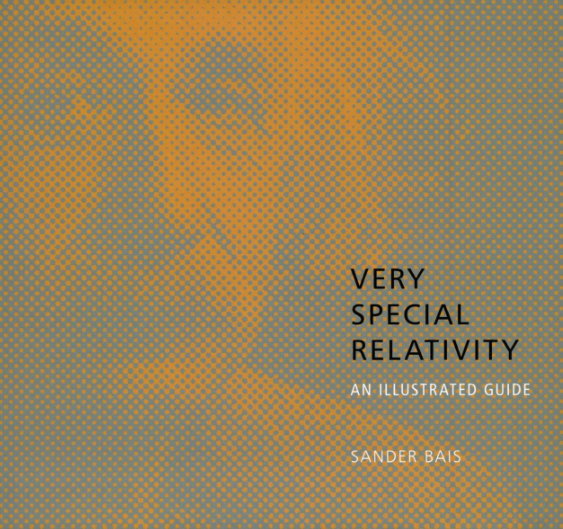
\includegraphics[width=.8\textwidth]{figures/vsr_cover.png}
    \captionsetup{font={scriptsize,sf}}
    \caption{How to learn special relativity.}
    \label{fig:VSR:cover}
\end{marginfigure}
\begin{marginfigure}%[th]
    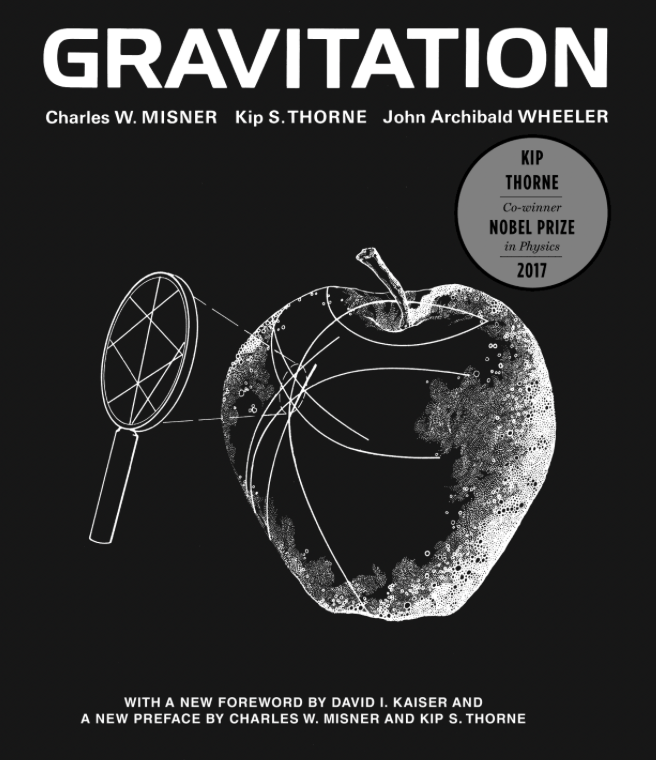
\includegraphics[width=.8\textwidth]{figures/MSW_cover.png}
    \captionsetup{font={scriptsize,sf}}
    \caption{Published 50 years ago---right around when the Standard Model was established---\tacro{MSW} is still one of the most insightful places to learn and re-learn relativity. }
    \label{fig:MTW:cover}
\end{marginfigure}

My favorite reference to appreciate the geometric structure of special relativity is the book \emph{Very Special Relativity}\autocite{bais2007very}. It looks like a miniature coffee table book, but it is a perfect book for physics students who have completed their lower-level coursework.\sidenote{If you can derive every result in the book then you are ready to take general relativity. You should be able to do this over a winter break.}\sidenote{Do not confuse the title of this book with the Cohen--Glashow hypothesis, \arXiv{hep-ph/0601236}, which is a rather different thing.} Once you have mastered this, you can pick up your favorite general relativity textbook for a bit more of the mathematical formalism. Some suggestions: Hartle\autocite{Hartle:2003yu}, Schutz\autocite{schutz2009first}, and Carroll\autocite{Carroll:2004st}. I would be remiss not to also mention the beautiful and elegant tome known lovingly as \acro{MSW}\autocite{misner2017gravitation}; a book so beloved that it had its own 50$^\textnormal{th}$ anniversary celebration.\footnote{\url{https://www.youtube.com/watch?v=a-4-IPBNV60}}



\section{The metric of spacetime}

The metric for spacetime without gravity is the four-dimensional Minkowski metric \eqref{eq:Minkowski:metric}. For the purposes of most of these examples, we will switch between the four-dimensional Minkowski metric and a simpler two-dimensional case with one dimension of time and one dimension of space.\sidenote{The simplified case is sufficient for motion along a single direction.} 

\begin{example}[West coast versus east coast]
There are two choices for the Minkowski metric:
\begin{align}
    g_{\mu\nu} &= 
    \begin{pmatrix}
        1 & & & \\
        & -1 & & \\
        & & -1 & \\
        & & & -1 
    \end{pmatrix}
    & \text{or}&
    &
    g_{\mu\nu} &= 
    \begin{pmatrix}
        -1 & & & \\
        & 1 & & \\
        & & 1 & \\
        & & & 1 
    \end{pmatrix} \ .
\end{align}
These are known as the mostly-minus (or ``west coast'') convention and the mostly-plus (or ``east coast'') convention respectively. One of the most diabolically frustrating open debates in physics is which of these equivalent metrics is more convenient. Some physicists like the mostly-minus metric because the norm of the four-momentum of a physical particle is positive. Others like the mostly-plus metric because the spatial components match the Euclidean metric. Whichever one you use, you pay the price somewhere else. As a particle physicist, I impose the mostly-minus metric.
\end{example}

Sometimes we write four-component vectors in a two-component shorthand. This is something I do for spacetime to separate the temporal from the spatial components of the four-vector.\sidenote{You may be a bit annoyed because it mixes up some of our notation.} In this notation, I may write a four-vector in Minkowski space as follows:
\begin{align}
    v^\mu = 
    \begin{pmatrix}
    v^0\\
    \vec{v}    
    \end{pmatrix} \ ,
\end{align}
where $\vec{v}$ is a three-vector is simply a number. However, the notation above also generalizes to different numbers of spatial dimensions.


\section{Natural Units}

There's one more convention that is useful in this business: \textbf{natural units}.\sidenote{Natural units are not strictly necessary for special relativity, but I find that if I do not use natural units I end up making errors all over the place.} This has nothing to do with linear algebra, but it does make our lives significantly easier. For our purposes, natural units is the following:
\begin{align}
    c = 1 \ .
\end{align}
Here $c$ is the speed of light, which usually has units of length divided by time. In natural units, we use the universal constant $c$ to convert between the two. Astronomers are already used to this: they measure distances in light years: the distance that a photon travels in one year, $d = c\times(1~\text{year})$. In natural units, we would just say `year.' In particle physics we also set Planck's constant $\hbar = 1$ which lets us convert between energy and time, but for our purposes it is sufficient to leave $c$ implicit. 

Natural units make our notation easier because we want the components of a four-vector to have the same units. It is silly to talk about a displacement four-vector\sidenote{Recall from Section~\ref{sec:no:position:vectors} that position vectors do not make sense, but relative positions do make sense as vectors.} $\Delta x^\mu$ if $\Delta x^0$ has units of seconds and $\Delta x^i$ has units of meters. This is even more perverse when we do a `rotation' between space and time (called a \emph{boost}). If we rotate in space, we know what it means when $\Delta x'^1 = \cos\theta \Delta x^1 + \sin\theta \Delta x^2$. This is because every term has the same dimensions. What does it mean to write $\Delta x'^0 = a \Delta x^0 + b \Delta x^1$ when $\Delta x^0$ is in seconds and $\Delta x^1$ is in meters? (We sort out the coefficients $a$ and $b$ below.) So one usually writes 
\begin{align}
    \Delta x^\mu = 
    \begin{pmatrix}
        c\Delta t \\ \Delta x \\ \Delta y \\ \Delta z
    \end{pmatrix} \ .
\end{align}
Maybe you don't mind that factor of $c$ in there? Things get annoying again when we write down four-momenta, whose time-like component is an energy. In order for the energy of a particle to have the same units as the three-momentum, we need to divide by $c$. Thus we write
\begin{align}
    p^\mu = 
    \begin{pmatrix}
        E/c \\
        p^1\\
        p^2\\
        p^3
    \end{pmatrix} \ .
\end{align}
In order to avoid all of these factors of $c$---you can always replace them at the end of a calculation by requiring dimensional consistency---we can simply set $c=$ so that
\begin{align}
    \Delta x^\mu &= 
    \begin{pmatrix}
        \Delta t \\ \Delta x \\ \Delta y \\ \Delta z
    \end{pmatrix}
    &
    p^\mu &= 
    \begin{pmatrix}
        E \\
        p^1\\
        p^2\\
        p^3
    \end{pmatrix} \ .
    \label{eq:momentum:4vec}
\end{align}
Because we are using units where $c=1$, the maximum velocity is 1. For historical reasons, we refer to the relative velocity between frames as $\beta = v/c$. In natural units, $\beta = v$ and $|\beta| \leq 1$.  


\section{Isometries of Minkowski spacetime}\label{sec:Lorentz:transformations}

% \section{Lorentz Transformations}\label{sec:Lorentz:transformations}

A \textbf{reference frame}\index{reference frame} is a basis for the vector space that represents what an observer may see. In ordinary Euclidean space, two frames may differ due to their relative orientation: if you are facing north, then the basis of `forward' and `to your right' means something different than if you were facing east. In relativity, in addition to rotations, observers in relative motion to one another also have different basis vectors. This, in turn, leads to different measurements of space and time when two observers are in relative motion.

How do you relate vector quantities between different reference frames? A particle may have some four momentum $p$.\sidenote{As per convention, we do not use bra-ket notation in relativity. I also reserve the typical vector notation $\vec{p}$ for the three-vector part of a four vector. It thus falls on you to determine from context whether $p$ refers to a four-momentum or the square root of its length, $p=\sqrt{p^\mu p_\mu}$. Sometimes we revert to component notation and write $p^\mu$ to mean the entire four-vector. Sorry, I could not think of a better alternative that would not stray too far from standard notation.} The \emph{components} of $p$ depend on the reference frame of the observer. We measure the components to be $p^\mu = (p^0, p^1, p^2, p^3)$. Another observer in another reference frame measures components $p'^\mu=(p'^0, p'^1, p'^2, p'^3)$. These components are related by a \textbf{Lorentz transformation}\index{Lorentz transformation}:
\begin{align}
    p^\mu = \Lambda\aij{\mu}{\nu}p'^\nu \ .
\end{align}
If we align the spatial parts of each observer's coordinate system so that their relative motion is in the $z$ direction, then the components of the Lorentz transformation are
\begin{align}
    \Lambda\aij{\mu}{\nu} =
    \begin{pmatrix}
        \gamma & & & \beta\gamma\\
        & 1 & &  \\
        & & 1 &  \\
        \beta\gamma &  &  & \gamma
    \end{pmatrix}
    \ . 
    \label{eq:Lorentz:in:z}
\end{align}
You should think about this as an analog of the rotation matrix in Euclidean space.\sidenote{The relation is as follows. Rotations are the isometries of Euclidean space: they are the transformations that preserve the dot product. Lorentz transformations are the isometries of Minkowski space: they are the transformations that preserve the metric. In both cases, the isometries are the allowed transformations that preserve the spacetime structure as encoded by the metric.} Here $\beta$ is the relative velocity between the two frames. If our coordinates are the unprimed coordinates and the other observer measures the primed coordinates, then $\beta$ is the other observer's velocity that we measure in our unprimed frame. 
\begin{exercise}
Check that \eqref{eq:Lorentz:in:z} is a transformation from frame $\mathcal O'$
 to frame $\mathcal O$, where $\mathcal O'$ is moving in the $+\hat{z}$ direction relative to the $\mathcal O$. Show that the inverse of $\Lambda$ simply swaps the sign of $\beta$. 

I often confuse myself about whether the $\gamma \beta$ terms should have a positive or negative sign in front of them. You can return to this thought-experiment to cross check  the sign of $\beta$ for yourself.
\end{exercise}
\begin{example}
A nice way to see the relation between Lorentz transformations and boosts is to note that we may write the boost parameter as \textbf{rapidity}\index{rapidity} $\eta$ defined through the identification:
\begin{align}
    \Lambda[\eta] = 
    \begin{pmatrix}
        \cosh \eta & \sinh \eta \\
        \sinh \eta & \cosh \eta
    \end{pmatrix}
    =
    \begin{pmatrix}
        \gamma & \beta\gamma \\
        \beta \gamma & \gamma
    \end{pmatrix} \ .
\end{align}
Compare this to a rotation matrix,
\begin{align}
    R(\theta) &=
    \begin{pmatrix}
        \phantom{+}\cos \theta & -\sin\theta \\
        \phantom{+}\sin \theta & \phantom{+}\cos\theta
    \end{pmatrix} \ .
    \label{eq:eg:rotations}
\end{align}
Observe the key relations:
\begin{align}
    \cosh^2 \eta - \sinh^2 \eta &= 1\\
    \cos^2 \theta + \sin^2 \theta &=1 \ .
\end{align}
Here we appreciate the critical minus sign that is the difference between space and time.\sidenotemark
\end{example}
\sidenotetext{The connection between Lorentz transformations and rotations is further explicit in the so called Pauli-metric formalism where the time-component of a four-vector is \emph{imaginary}. In that formalism the metric is proportional to the identity and both Lorentz transformations and rotations take the form \eqref{eq:eg:rotations}.}

What about the transformation of lower index objects, like $p_\mu$? We can motivate based on what we know physically. But first, it is useful to review the case of simple rotations:
% 
\begin{example}[Transformation of row vectors]\label{eg:row:vector:transform}
Consider a Euclidean three-vector $\vec{v} = (v^1, v^2, v^3)^\trans$ and a Euclidean row vector, $\row{w} = (w_1, w_2, w_3)$. You know that the contraction these two objects is a number that is \emph{invariant}.
\begin{align}
    \row{w}\vec{v} = w_1v^1 + w_2 v^2 + w_2 v^2 .
\end{align}
In fact, if $\row{w} = \vec{w}^\trans$, then $\row{w}\vec{v}$ is simply the inner product $|\vec{w}||\vec{v}|\cos\theta$. At any rate, the contraction $w_i v^i$ carries no indices and is a pure scalar quantity. That means it does not transform under rotations. However, we know that $\vec{v}$ \emph{does transform under rotations},
\begin{align}
    \vec{v}&\to R(\theta)\vec{v} 
    \ ,
\end{align}
with $R(\theta)$ given in \eqref{eq:eg:rotations}.
That means $\row{w}$ should also transform in a way to compensate the $\vec{v}$ transformation and keep $\row{w}\vec{v}=w_iv^i$ constant. Call this transformation $S(\theta)$. By the rules of matrix multiplication, $S(\theta)$ must act from the right:
\begin{align}
    \row{w} \to \row{w}S(\theta) \ \,
\end{align}
but from the index perspective the order does not matter:
\begin{align}
    w_i \to w_i S(\theta)\aij{i}{j} =  S(\theta)\aij{i}{j} w_i \ .
    \label{eq:order:of:terms:in:summation}
\end{align}
This is because each term in the sums on the right-hand sides of \eqref{eq:order:of:terms:in:summation} are just multiplication of two numbers. \emph{Make sure you understand this.}

The statement that $\row{w}\vec{v}$ is constant under rotations is
\begin{align}
    \row{w}\vec{v} \to \row{w}S(\theta)R(\theta)\vec{v}
    = 
    R(\theta)\aij{i}{\ell} S(\theta)\aij{k}{i} w_k v^\ell
\end{align}
so that we requre:
\begin{align}
      R(\theta)\aij{i}{\ell} S(\theta)\aij{k}{i}
      =
      S(\theta)\aij{k}{i}R(\theta)\aij{i}{\ell}
      =
      \delta\aij{k}{l} \ ,
      \label{eq:SR:RS:inverses}
\end{align}
or in other words, as matrices, $S(\theta)R(\theta) = 1$. Note that while it turns out to also true that $R(\theta)S(\theta) = 1$, \eqref{eq:SR:RS:inverses} is \emph{only} telling us that $S(\theta)R(\theta) = 1$ because when we write this index contraction was a matrix multiplication, the order matters: we have to make sure contracted indices are consecutive.

We thus conclude that
\begin{align}
    S(\theta) = R(\theta)^{-1} = R(-\theta) = R(\theta)^\trans \ .
\end{align}
So we demonstrate something very important: row vectors like $\row{w}$ `rotate oppositely' from column vectors like $\vec{v}$. All of this is simply a rehash of what we discussed in Section~\ref{sec:transformation:under:symmetries}.
\end{example}

The lesson from the above example is that lower indexed objects transform with the \emph{inverse transformation} as upper indexed objects. Thus if $p^\mu \to \Lambda\aij{\mu}{\nu}p^\nu$, we must have
\begin{align}
    p_\mu \to (\Lambda^{-1})\aij{\nu}{\mu} p^\nu\ .
\end{align}
Check to make sure that you agree with the position of the indices. It is $(\Lambda^{-1})\aij{\nu}{\mu}$, not $(\Lambda^{-1})_{\mu}^{\phantom{\mu}\nu}$. 
%Refer back to Example~\ref{eg:row:vector:transform} if that is not clear.



\section{Example: Muon Decay}

Cosmic rays can produce muons when they hit the upper atmosphere about 10 kilometers above the surface of the Earth.\sidenote{This sub-section is copied from my Physics 17 (2023) notes and is adapted from an example in Griffiths.} These muons are highly relativistic, with a velocity of $\beta = 0.9999$. See Fig.~\ref{fig:muons}. We know from laboratory experiments that the lifetime of a muon \emph{at rest} is 2 microseconds. Based on the simple estimate $d=c\tau \approx 600$~meters, we would not expect any muons to reach the surface of the Earth. However, not only do large cosmic ray telescopes have dedicated muon detectors, but you can make your own citizen science muon detector\sidenote{\url{https://muonpi.org}}. What gives?
\begin{marginfigure}%[tb]
    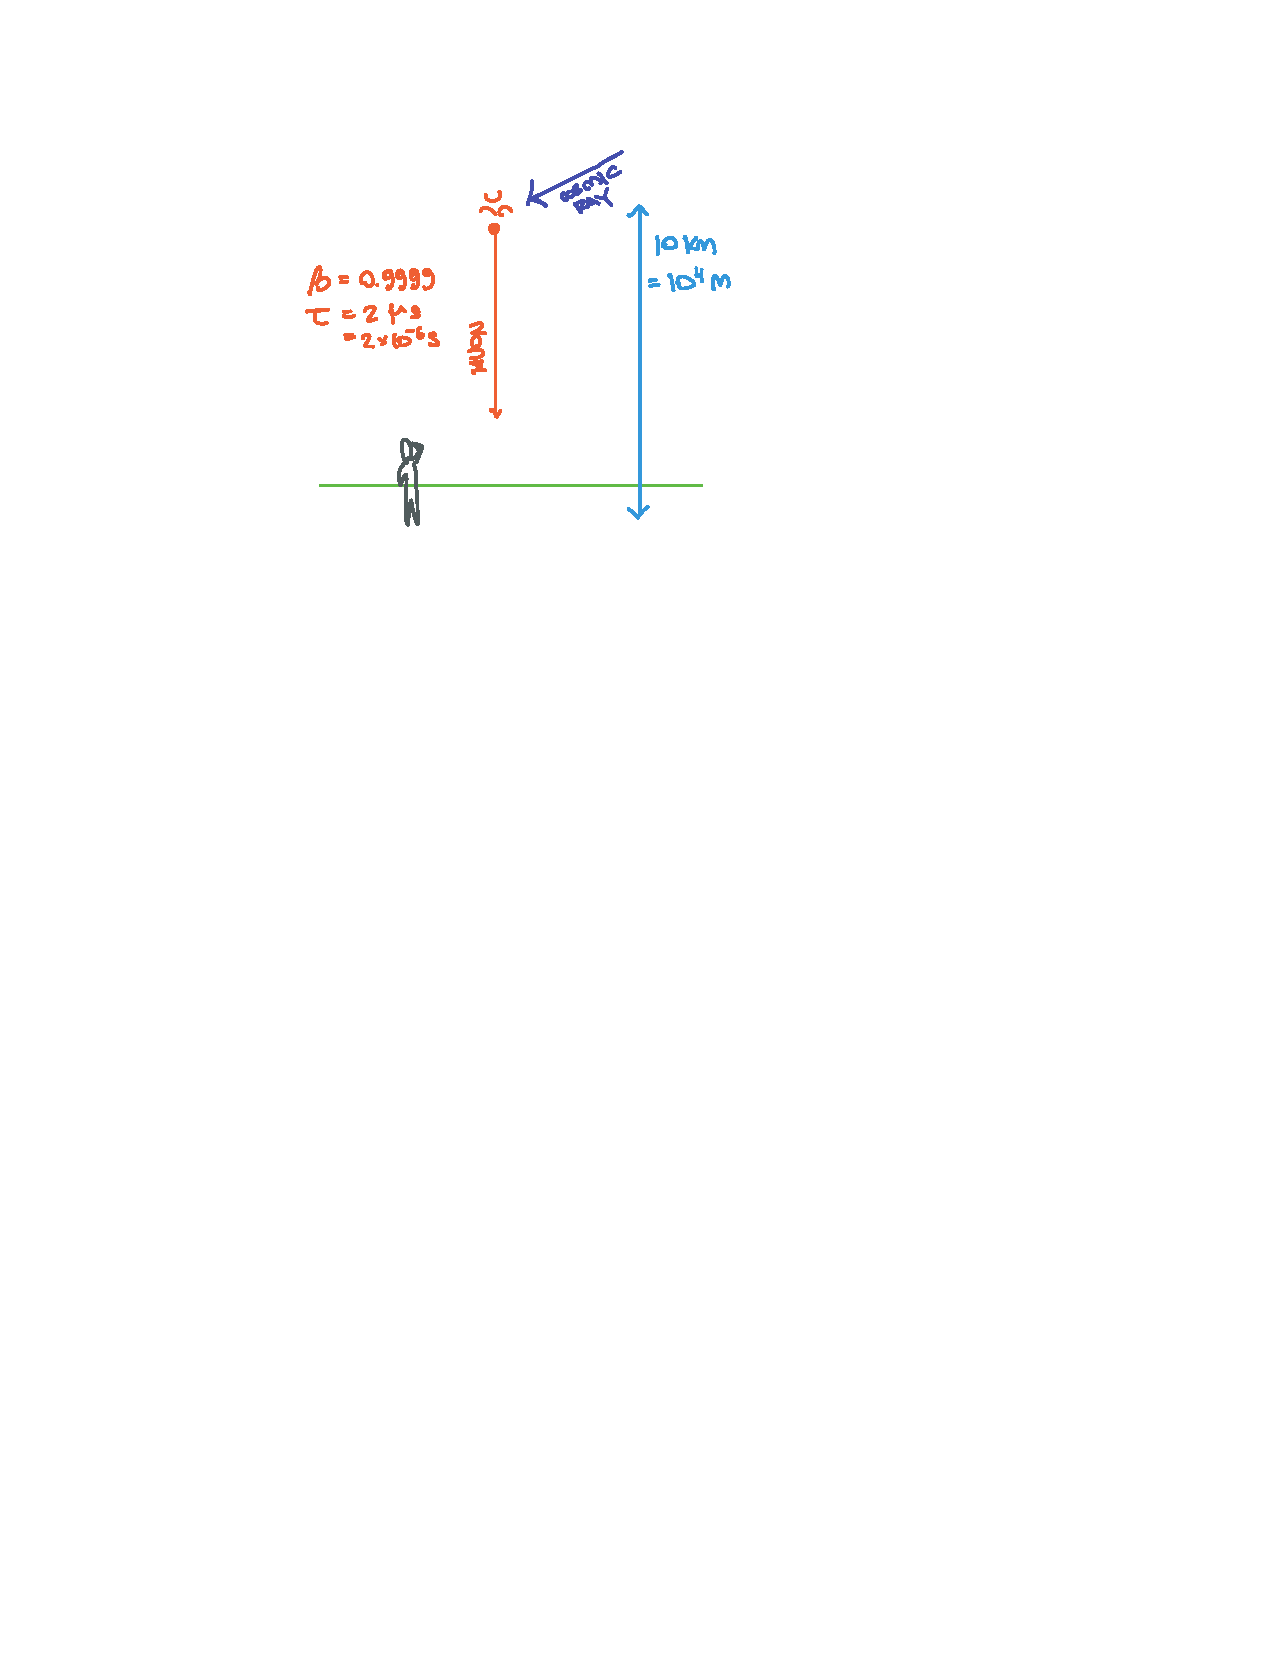
\includegraphics[width=\textwidth]{figures/muon.pdf}
    \captionsetup{font={scriptsize,sf}}
    \caption{Very technical sketch of a muon produced in the upper atmosphere heading towards earth. \label{fig:muons}} 
\end{marginfigure}
Here are the facts:
\begin{itemize}
    \item Both the observer on Earth and the muon agree that their relative velocity is $|\beta| = 0.9999$. 
    \item The muon's lifetime is known in the muon's rest frame. 
    \item The distance from the surface of the Earth to the upper atmosphere is known in the Earth's rest frame. 
\end{itemize}
The Lorentz transformation between the muon frame and the observe frame mix up space and time separations. We can only express the distance or time that the muon travels by calculating in the same reference frame. 

% \begin{figure}[tb]
%     \centering
%     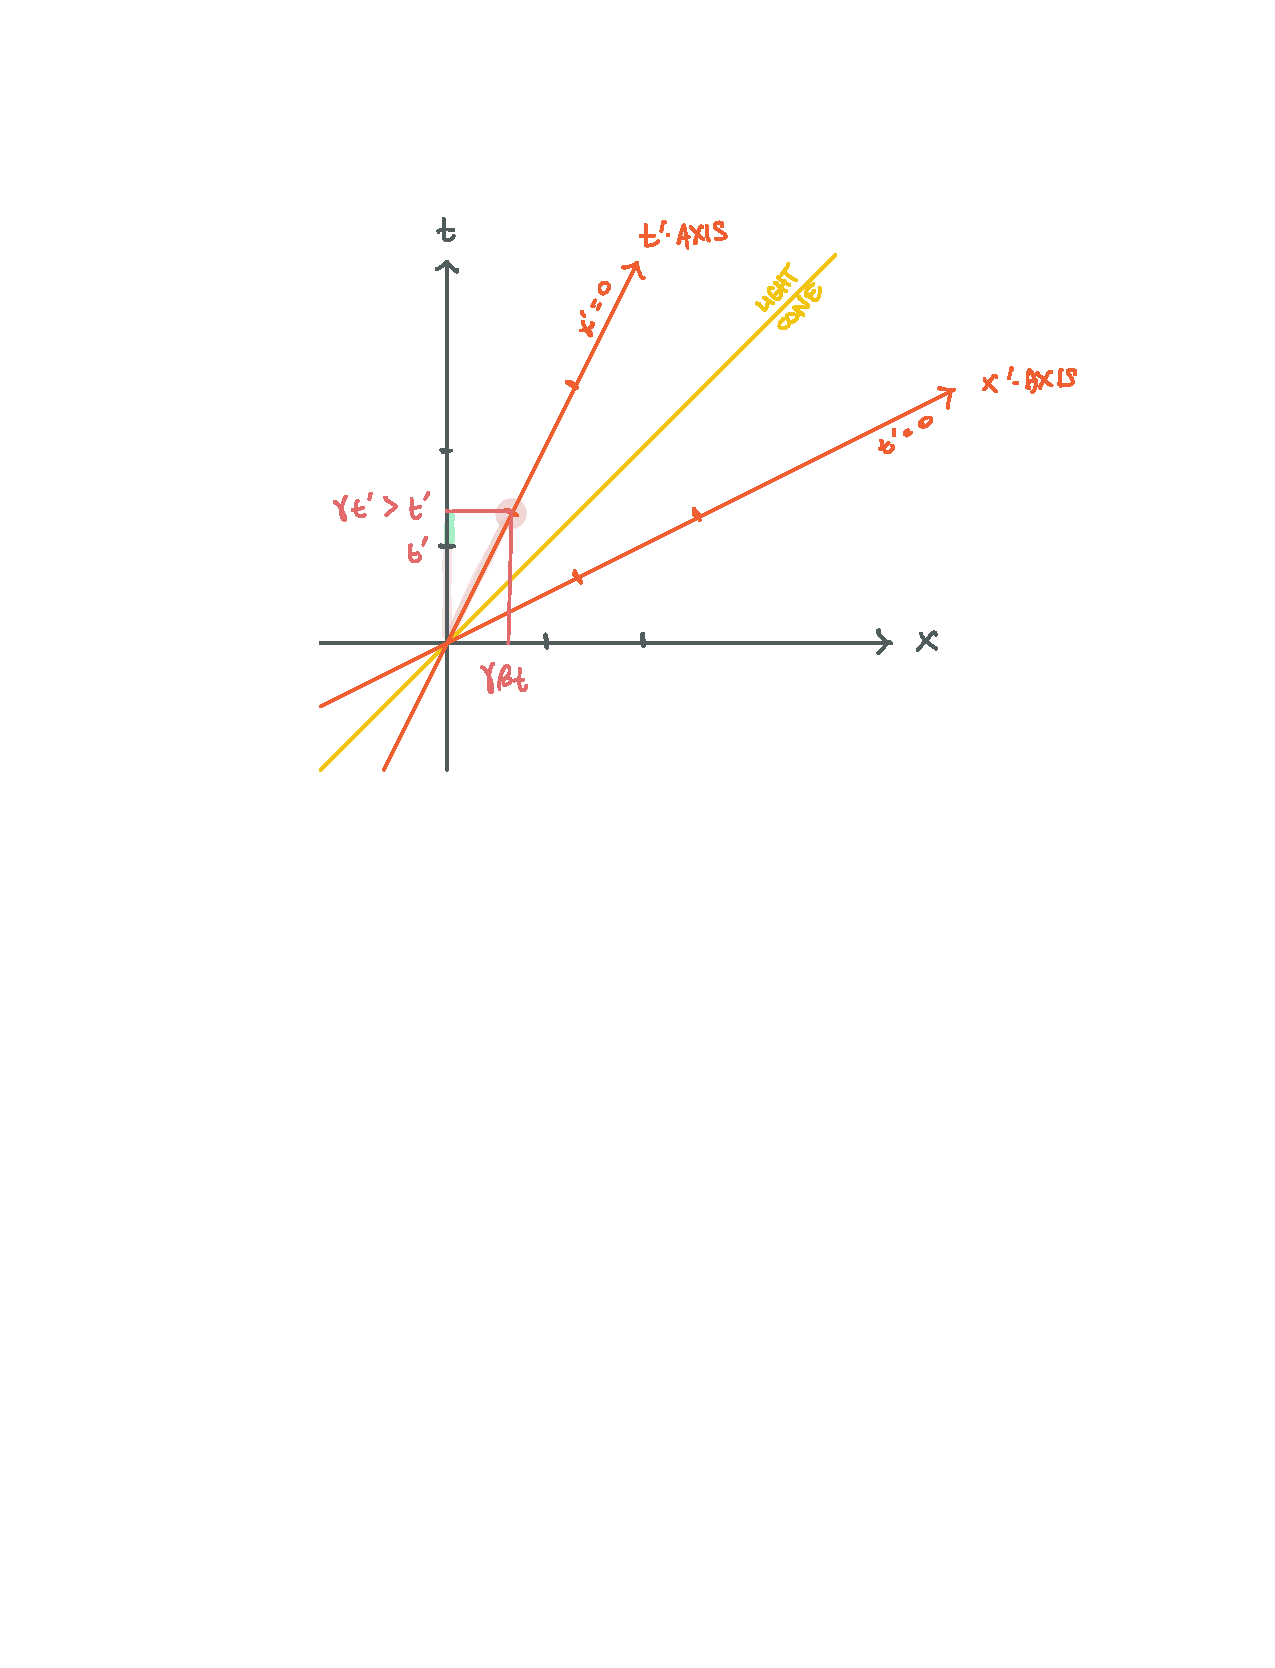
\includegraphics[width=.48\textwidth]{figures/rel_time_dil.pdf}
%     \quad
%     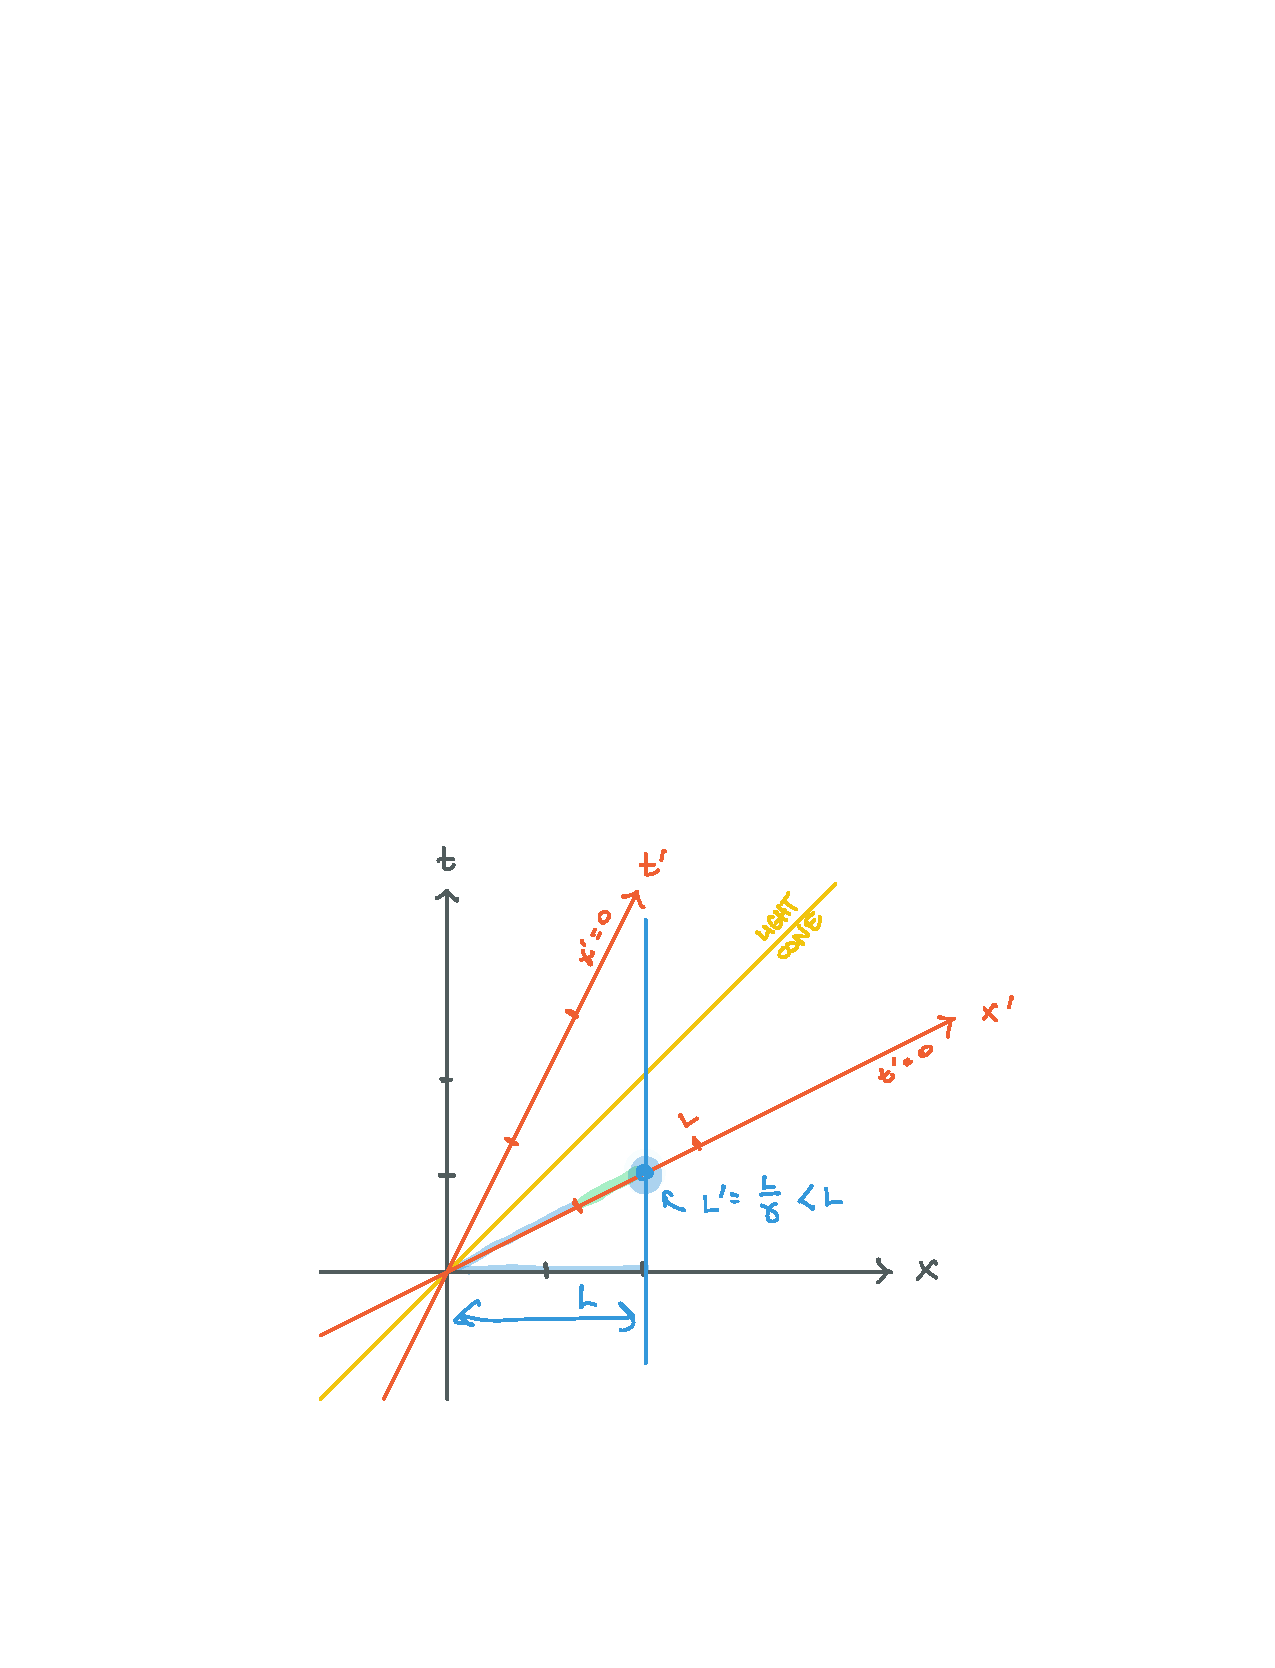
\includegraphics[width=.48\textwidth]{figures/rel_len_contractino.pdf}
%     \caption{Left: the muon's lifetime is time-dilated in the Earth's frame. Right: the distance from the surface of the Earth to the upper atmosphere is length contracted in the muon's frame. }
%     \label{fig:re:dilation}
% \end{figure}

First let us consider calculating everything in the Earth's reference frame. This is shown on the left of Fig.~\ref{fig:re:dilation}. This means we have to take the muon's lifetime in the muon's rest frame and convert it into a lifetime in the Earth's frame. In the muon's frame the lifetime is simply 
\begin{align}
    \Delta x'^\mu &= 
    \begin{pmatrix}
    \tau \\ 0     
    \end{pmatrix} \ 
    &
    \Delta x^\mu &=
    \begin{pmatrix}
    \gamma \tau \\ \gamma\beta \tau    
    \end{pmatrix} \ ,
\end{align}
where we have noticed that the muon lifetime is a displacement along the $t'$ axis. We find that the lifetime in the Earth's frame is actually larger than the lifetime in the muon rest frame: $t = \gamma \tau$. There is also a spatial component, but this is no surprise: in the Earth frame the muon is moving, so when the muon decays it is in a different position. 

How much is the muon's lifetime \emph{time dilated}? We plug $\beta$ into the expression for $\gamma = (1-\beta^2)^{-1/2}$. We find\footnote{There's a cute trick here: $\beta^2 = (1-\epsilon)^2 \approx 1- 2\epsilon$ by Taylor expanding in the small number $\epsilon = 10^{-4}$.} that to one significant figure, $\gamma = 100$. This means that the time for the muon decay in the Earth's frame is $2\times 10^-4$~seconds, which means that it travels approximately $d=60~$km, which is larger than the distance from the upper atmosphere to the surface. As a sanity check: this is exactly the value in the spatial component of $\Delta x^\mu$.

Great: so one story is that relativistic muons have lifetimes that are much larger than their at-rest lifetime. This means that to the observer on earth, the muon simply lives longer than we would expect from measurements of muons at rest. There are, however, (at least) two sides to every good story. What does the muon see?

In the muon's rest frame, the muon \emph{knows} that it goes \emph{kaput} in 2~microseconds. It sees the surface of the Earth approaching it with velocity $\beta = 0.9999$. By now you can guess that must change: the measurement in the Earth's frame---that the height of the upper atmosphere is 10~km---must be different in the muon's frame. And in fact, the muon must measure the distance of the rapidly approaching Earth to be much smaller than 10~km. How does this \emph{length contraction} work? 

We show this on the right side of Fig.~\ref{fig:re:dilation}.
\begin{marginfigure}
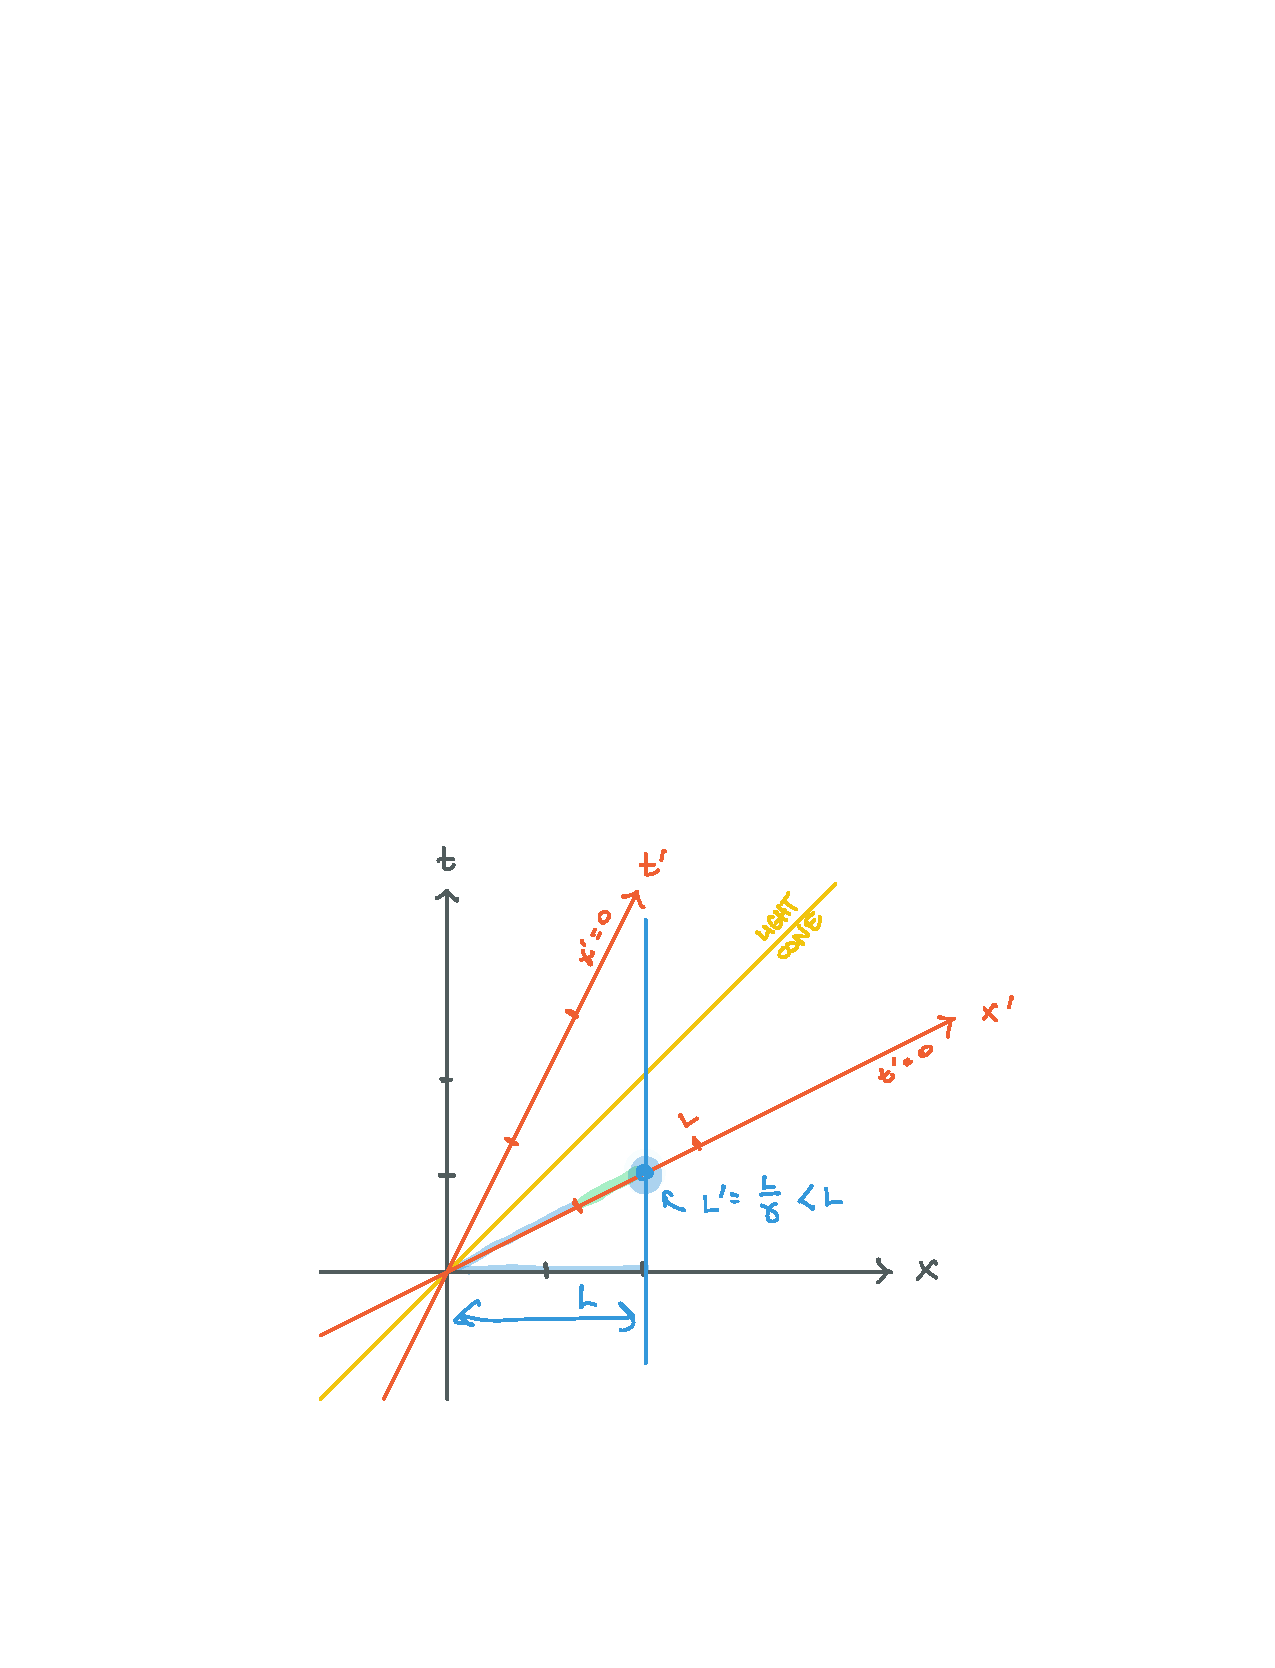
\includegraphics[width=\textwidth]{figures/rel_len_contractino.pdf}
\captionsetup{font={scriptsize,sf}}
\caption{The distance from the surface of the Earth to the upper atmosphere is length contracted in the muon's frame.
    \label{fig:re:dilation}
}
\end{marginfigure}
Note that now we have a measurement in the Earth frame (a vertical line denoting a fixed distance) that we want to project onto the muon frame (red axes). In the Earth frame, we denote the distance by two unit ticks in the spatial direction. In the muon frame, this line intersects the $x'$ axis with \emph{less} than two ticks.

\begin{exercise}
Using the Lorentz transformation laws, show that the distance from the muon to the surface of the Earth at the moment of the muon's creation is $L'=L/\gamma$ where $L=10$~km is the distance in the Earth frame. 
\end{exercise}

% \section{The metric tensor}

% The \textbf{inner product} (or dot product) is a machine that takes two vectors and outputs a number. It is manifested by a tensor called the metric, which has two lower indices:
% \begin{align}
%     \langle p,q\rangle = p\cdot q = g_{\mu\nu}p^\mu q^\mu \ .
% \end{align}
% In special relativity the metric is conventionally written as $\eta_{\mu\nu}$ and has a simple form in Cartesian coordinates:
% \begin{align}
%     \eta_{\mu\nu} = 
%     \begin{pmatrix}
%         1 & & & \\
%         & -1 & & \\
%         & & -1 & \\
%         & & & -1
%     \end{pmatrix}
%     = \textnormal{diag}(1,-1,-1,-1) \ .
% \end{align}
% Some physics tribes\sidenote{Particle physicists use the `West coast' or `mostly minus' notation. It is usually relativists and formal theorists who use the East coast/mostly plus convention. A third convention, the `Pauli convention' uses a metric proportional to the identity but with the timelike component imaginary $x^4 = ix^0$. In that notation, boosts look like complex rotations. See Appendix F of \emph{Diagrammatica}\footnotemark by Veltman for a discussion.}\footnotetext{\cite{Veltman:1994wz}} use a different convention, $\eta_{\mu\nu} = \text{diag}(-1,1,1,1)$. The choice of whether the spatial or temporal pieces pick up the minus sign is a convention---while the intermediate steps of any calculation differ by these annoying signs, any physical result is independent of the convention.\sidenote{I am hopelessly entrenched in the mostly minus tribe. If I were being honest, I think the mostly-plus metric is probably easier to start learn if you were starting from scratch. But I intend to run with team mostly-minus until I die.}


% The metric has an inverse, $g^{\mu\nu}$ or $\eta^{\mu\nu}$ in special relativity. It has two upper indices and satisfies
% \begin{align}
%     g_{\mu\nu}g^{\mu\nu} = g^{\mu\nu}g_{\mu\nu} = \delta^\mu_\nu \ .
% \end{align}
% We do not bother writing $(g^{-1})^{\mu\nu}$ because the height of the indices indicates precisely whether you are using the metric or inverse metric. In special relativity, the components of $\eta_{\mu\nu}$ and $\eta^{\mu\nu}$ are identical. Also observe that the Kronecker-$\delta$ has no distinction between first and second indices:
% \begin{align}
%     \delta^\mu_\nu =
%     \begin{cases}
%     1 & \text{if } \mu = \nu \\
%     0 & \text{otherwise} 
%     \end{cases}
%     \ .
% \end{align}
% The Kronecker-$\delta$ represents the components of the unit matrix, $\mathbbm{1}\aij{\mu}{\nu} = \delta^\mu_\nu$.


\section{Example: Alien measurement}
\label{sec:relativity:alien}


In special relativity there is an object called the four-velocity.\sidenote{This subsection borrows from my Physics 17 (2023) notes.} In our rest frame, our four velocity is
\begin{align}
    v^\mu = \begin{pmatrix}
        1\\ 0
    \end{pmatrix} \ .
    \label{eq:4:velocity:in:rest:Frame}
\end{align}
This literally means that when we are at rest, we are moving one second per second in the time direction. Objects moving relative to us have four velocities that are Lorentz transformations of the $v^\mu$ above. 

We notice that we can write the energy of a particle in a way that uses the inner product:
\begin{align}
    \langle v, p\rangle = p\cdot v = g_{\mu\nu} p^\mu v^\nu \ .
\end{align}
Of course, all this does is pick out the $p^0$ component, as we knew it had to. However, unlike writing $p^0$, the inner product $p\cdot v$ has no indices. It is a pure number and so it does not transform under Lorentz transformations. 

\begin{marginfigure}%[tb]
    \centering
    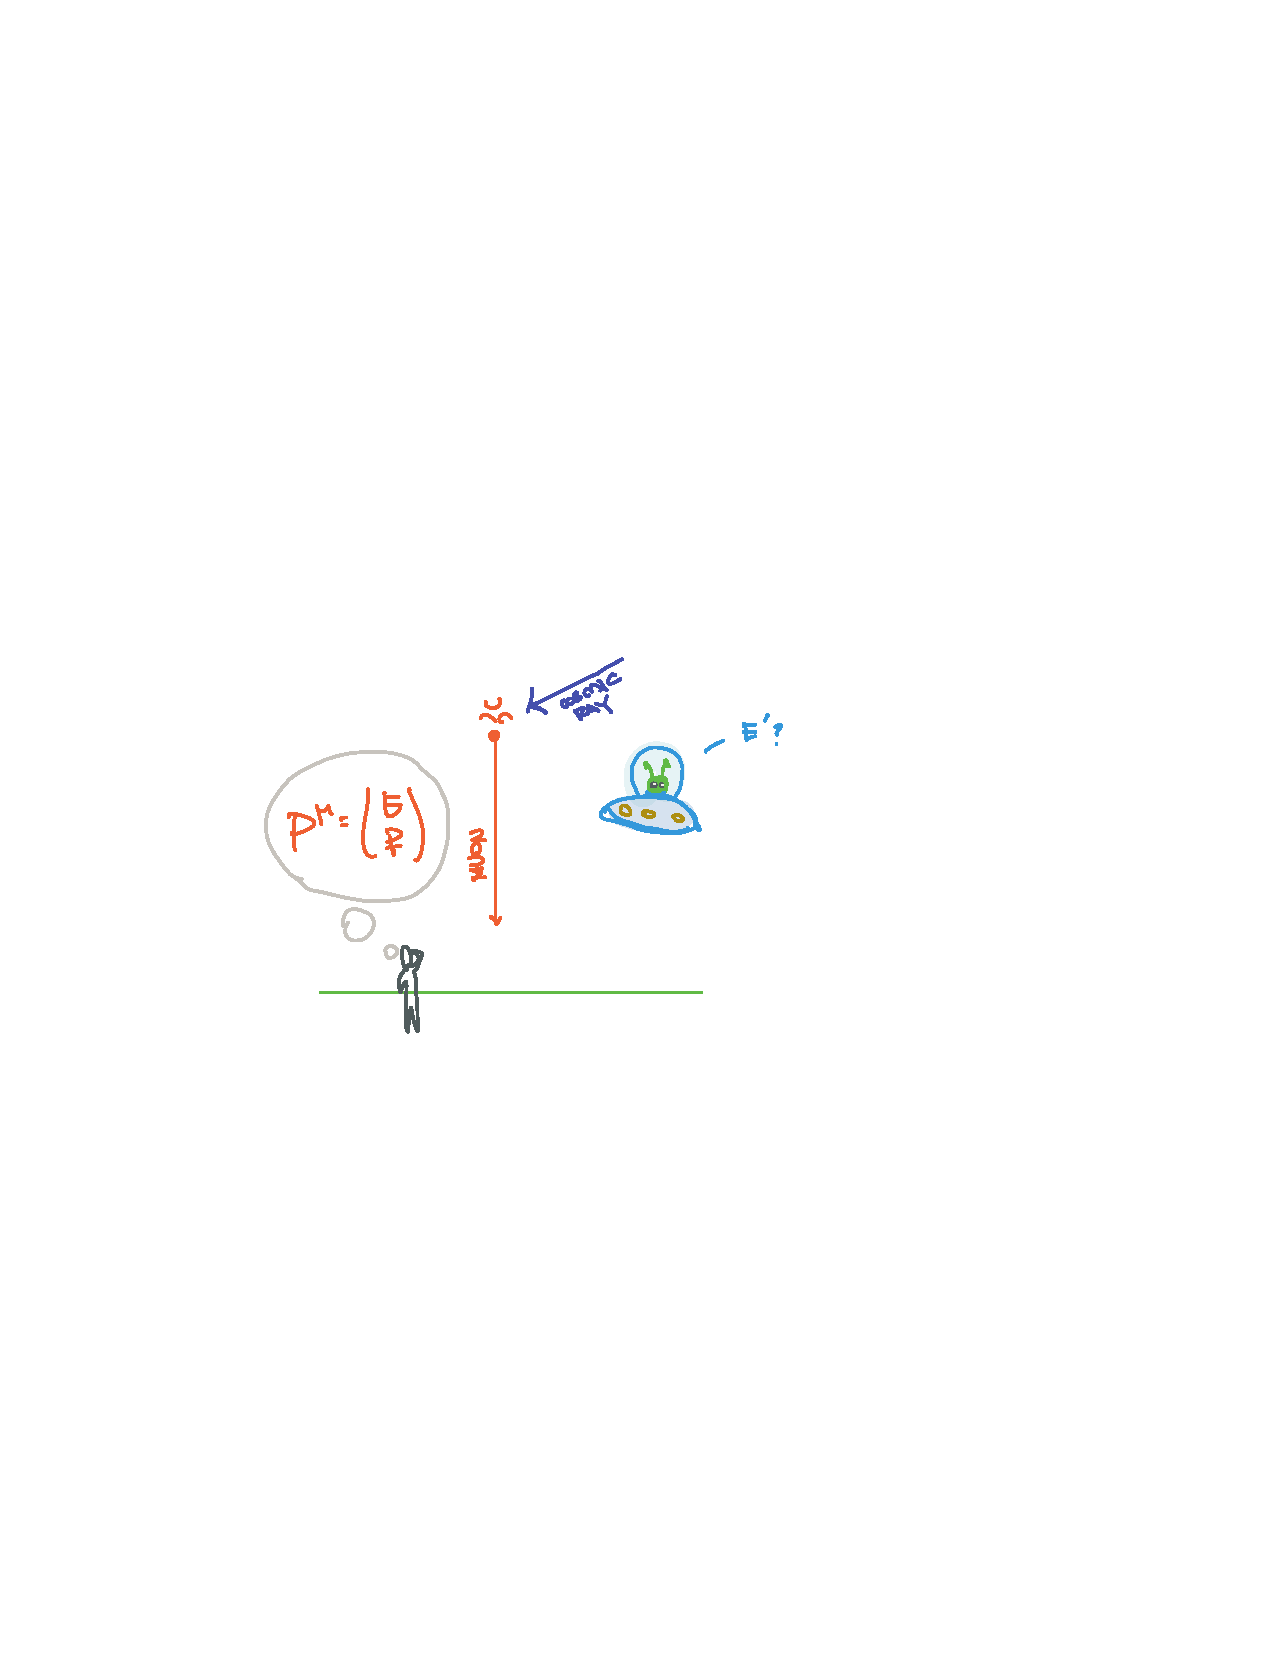
\includegraphics[width=\textwidth]{figures/alien.pdf}
    \captionsetup{font={scriptsize,sf}}
    \caption{You measure the four-momentum of a particle. What is the energy that an alien moving at some velocity $\beta$ relative to you measures?\label{fig:alien}}
\end{marginfigure}

At this point you wonder if we are simply reciting random facts that we have developed. Consider the following scenario illustrated in Fig.~\ref{fig:alien}.
%
% 
While you are measuring the particle energy $p^0 = E$, you notice an alien traveling relativistically with velocity $\beta$ relative to you. The alien has sophisticated equipment to measure the particle energy, and you know that the alien measures a different energy $E'$. How can you determine what the alien measures?

One way to do this is to calculate the full Lorentz transformation between your frame and the alien frame. That is tedious. It turns out that we can use the four-velocity as a useful trick. All objects with mass have a four-velocity equal to \eqref{eq:4:velocity:in:rest:Frame} in their rest frame. This means that the alien measures the particle to have energy $v_\text{alien}\cdot p_\text{alien}$, where the subscript `alien' means that these are all calculated in the alien's frame.

We now remember that $v_\text{alien}\cdot p_\text{alien}$ is a number. It does not matter what frame we calculate it in. Thus it is equivalent to the same dot product measured in our frame:
\begin{align}
E'=
    v_\text{alien}\cdot p_\text{alien} = v\cdot p \ ,
\end{align}
where the right-hand side is the alien four-velocity and the particle four-momentum as measured in our frame. The alien four-velocity is simply a Lorentz transformation of \eqref{eq:4:velocity:in:rest:Frame}. More practically, it is something that you can measure in your own frame. 


\begin{exercise}
Rephrase everything in this example in terms of the inner product in Minkowski space. Bonus if you use the word `projection.'
\end{exercise}




\section{Velocity transformations}

When I was first learning special relativity, I had somehow internalized the idea that transforming velocities between references frames is hopelessly difficult. I suspect that this is confusion was because I was learning the physical effects of relativity before learning the geometric foundation of the effects. Armed with a modicum of mathematical sophistication, deriving the velocity transformation is simple. 

First, let us define the spacetime trajectory of a particle $x^\mu(\lambda)$. This is a curve in spacetime that relates every time $x^0(\lambda)$ to a position $x^i(\lambda)$. $\lambda$ is called an \textbf{affine parameter}\index{affine parameter}, which is just a fancy name for some number that tells you where in spacetime the particle is. We may choose coordinates where $\lambda=0$ corresponds to $x^\mu = 0$. This affine parameter is just some tool that we use to describe the curve: it is \emph{not} a time variable,\sidenote{In relativity problems it can be convenient to \emph{choose} $\lambda$ to be the proper time, the time that the particle would measure in its own rest frame.} in fact, $\lambda$ does not even need to have units. 

The velocity is an infinitesimal displacement in space divided by the corresponding infinitesimal displacement in time. The affine parameter is assumed to be a `nice' map from $\mathbbm{R}$ to spacetime positions, so values $\lambda$ and $\lambda + \varepsilon$ for small $\varepsilon \ll 1$ correspond to nearby points in the particle's spacetime trajectory. Let us look at velocities at the spacetime point $\lambda = 0$. This is convenient because we know that Lorentz transformations map the origin to the origin: $\Lambda 0 = 0$, where here $0$ is the four-vector with all zero elements. That means that if the trajectory has coordinaets $x^\mu(\lambda)$ in some coordinate system, the velocity is\sidenote{It is important that the numerator and denominator are \emph{differences} in positions because---as I say often---\emph{there is no such thing as a position vector}.}
\begin{align}
    v^i \defeq 
    \lim_{\epsilon\to 0} \frac{x^i(\epsilon) - x^i(0)}{x^0(\epsilon)- x^0(0)} 
    =
    \lim_{\epsilon\to 0} \frac{x^i(\epsilon)}{x^0(\epsilon)}
    \ .
    \label{eq:SR:velocity:def}
\end{align}
Let us simplify the problem further by working in (1+1)-dimensions so that $i=1$ only. We write $v\defeq v^i$. In this case we perform a Lorentz transformation by
\begin{align}
    \Lambda\aij{\mu}{\nu} =
    \begin{pmatrix}
        \pp \gamma & -\gamma\beta \\
        -\gamma\beta & \gamma
    \end{pmatrix} \ .
\end{align}

What does the Lorentz transformation act on? It acts on the objects with indices. This means that the numerator and denominator or \eqref{eq:SR:velocity:def} each transform:
\begin{align}
    v \to v' =
    \frac{
        \gamma x^i - \gamma\beta x^0
    }{
        \gamma x^0 - \gamma\beta x^i
    }
    =
    \frac{
        v -\beta
    }{
        1 - \beta v
    } \ .
\end{align}
And that's it! The boost parameter $\beta$ is \emph{also} a velocity. Sometimes you see this written as $\beta = u$ to make it clear that $u$ and $v$ are objects of the same class.\sidenote{But in this calculaiton, they are \emph{not} of the same class: $v$ is the velocity that you want to write in the boosted frame, and $u$ is a transformation parameter---that happens to also be a velocity---that tells you how to get to the boosted frame.} Sometimes there is a sign difference $\beta \to -\beta$ so that there are no minus signs in the above expression. This is simply a choice of active versus passive transformation and does not change the transformation since $-1 < \beta < 1$. That is: the other sign convention is related to our convention by boosting in the opposite direction.



\begin{exercise}
Generalize\footnote{One of my favorite memories of my graduate education was when a particle physics lecturer used the phrase ``generalize to the case $N=3$. One of my good friends in the class, a relativist, started laughing. After seeing my confusion, he explained that $N=3$ is as specific a choice as $N=1$. The lesson, of course, is that often any specific choice $N>1$ shows the features of a generic choice of $N$. Since then, I smirk every time I catch myself saying `generalize to [some specific number].' Thanks to Prof.~Steffen Gielen for all the great times.} our expression for velocity transformations to (3+1)-dimensions. The key step is to recognize that the direction of the velocity need not align with that of the boost so that you must treat the parallel and perpendicular components separately. 
\end{exercise}


\begin{exercise}
Derive the transformation law for accelerations. You may work in the (1+1)-dimensional case.
\end{exercise}

\begin{exercise}
The \emph{relativistic relative velocity} is an idea that comes up often in astroparticle physics, though there are very few treatments that are both correct and complete. In Galilean physics, the relative velocity between two particles with velocities $\vec{v_1}$ and $\vec{v_2}$ is simply $\vec{v_1}-\vec{v_2}$. This is no longer true relativistically. Calculations for rates (cross sections) in collider physics, for example, often have a factor of the relative velocity of the particles in the two beams. If the particles in each beam are accelerated to nearly the speed of light, $|\vec{v_i}| \approx 1$ but have opposite directions $\vec{v_1} = - \vec{v_2}$, then the Galilean definition of relative velocity would have magnitude larger than the speed of light. Come up with a definition of the relativistic relative velocity by starting in the frame where one of the beam particles is at rest. For a insightful discussion with references, see Cannoni.\autocite{Cannoni:2013bza} While this idea is something that you would \emph{think} is standard, I only stumbled upon it fairly recently when a then-\acro{UCR} postdoc, Prof.~Aniket Joglekar, re-discovered it during a subtle calculation.\autocite{Joglekar:2020liw}
\end{exercise}

% \section{Tensors: the meaning of indices}


% The lightning-quick review of special relativity here is an example of tensor analysis in physics.\sidenote{Where can you learn more? I recommend my Physics 17 lecture notes. Want a more advanced version? Check out my Physics 231 lecture notes.} Tensors show up \emph{all over the place} in physics. Even in your lower division physics courses: did you ever wonder why it is called the moment of inertia \emph{tensor} and not the moment of inertia \emph{matrix}? Yes, there is a difference.\footnote{See e.g.\,\url{https://hepweb.ucsd.edu/ph110b/110b_notes/node24.html}}\sidenote{I am frustrated that few textbooks take a moment to explain the significance this difference.} For our purposes, we can think of a \textbf{tensor}\index{tensor} as an object that has an ordered number of indices. The indices each have a height, either upper or lower. 

% The order of the indices matters; if you want it takes precedence over the height of the index: 
% \begin{align}
%     T^{ij\phantom{k}\ell}_{\phantom{ij}k} \neq
%     T^{\phantom{k}ij\ell}_{k} \ .
% \end{align}
% If you have a metric, this is more clear since you can lower (or raise) all the indices, so that 
% \begin{align}
%     T^{ij\phantom{k}\ell}_{\phantom{ij}k} &= T^{ijm\ell}g_{mk}
%     \\
%     T^{\phantom{k}ij\ell}_{k}&=T^{mij\ell} g_{mk}
% \end{align}
% and you can see that $T^{mij\ell} \neq T^{ijm\ell}$.

% There are some equivalent ways of thinking about tensors. The most formally correct way is to think about them as \emph{multilinear maps} between vector spaces (or tensor products\sidenote{Given a vector space $V$, a tensor product $V\otimes V$ is two copies of the vector space.} thereof). Perhaps more practically, a tensor is an object that encodes information that transforms according to the height of the indices. Generalizing our rules from Section~\ref{sec:Lorentz:transformations}:
% % 
% \begin{newrule}[Tensor transformation]\label{rule:tensor:transform}
% If $T$ is a tensor with upper indices $i_1, \cdots, i_N$ and lower indices $j_1, \cdots, j_M$, then under a symmetry transformation $R(\theta)$, $T$ transforms as
% \begin{align}
%     T^{\cdots}_{\cdots} \to 
%     R(\theta)^{i_1}_{\phantom{i_1} k_1} 
%     \cdots 
%     R(\theta)^{i_N}_{\phantom{i_N} k_N}
%     (R(\theta)^{-1})^{\ell_1}_{\phantom{\ell_1}j_1} 
%     \cdots 
%     (R(\theta)^{-1})^{\ell_M}_{\phantom{\ell_M}j_M} T^{\cdots}_{\cdots} \ ,
% \end{align}
% where we have written $\cdots$ on the left hand side to mean `some arrangement of upper $i$ and lower $j$ indices,' while on the right the $\cdots$ mean `some arrangement of upper $k$ and lower $\ell$ indices.'

% In other words:
% \begin{itemize}
%     \item For each upper index, multiply by a factor of $R(\theta)$ and contract with the lower index of $R(\theta)$.
%     \item For each lower index, multiply by a factor of $R(\theta)^{-1}$ and contract with the upper index of $R(\theta)^{-1}$. Note that this is contraction with the \emph{first} index of $R(\theta)^{-1}$. 
% \end{itemize}
% \end{newrule}
% To apply the rule for Lorentz transformations, simply replace $R$ with $\Lambda$ and convert the indices into $\mu$s and $\nu$s. 

% We ultimately care about quantities that are \emph{invariant}\index{invariant} under Lorentz transformations. These are objects that everyone agrees upon, no matter what their reference frame. If you were to build a theory of nature, you would want the physical laws from that theory to be invariant with respect to reference frame---so the objects you would build that theory out of are naturally invariants. 





\section{Isometry}
\label{sec:spacetime:isometry}

How does one know that rotations are important symmetries in Euclidean space? This certainly comes from our own experience with physics---the laws of physics are rotationally invariant. In fact, we learn very quickly in our physics training to use rotational invariance to simplify problems. What about in special relativity? Historically, the Michelson--Morley non-observation\sidenote{Perhaps the most significant null result in science.} of aether---that is, the observation that the speed of light is constant---led us to realize that requirement that physics cannot depend on reference frame leads to a different class of symmetries. What characterizes these symmetries?

From a top-down perspective, rotations and their generalizations\sidenote{Such as Lorentz transformations in special relativity.} are \emph{isometries}. An \textbf{isometry}\index{isometry} is a symmetry of \emph{the form of the metric}. Specifically, it is a transformation---enacted by a matrix acting on vectors, for example---for which the \emph{components} of the metric do not change. With our conventions, special relativity requires that the components of the metric are $\eta_{\mu\nu} = \text{diag}(+,-,-,-)$; this means that the metric takes this form in \emph{any} reference frame. 


Ah! But we know that the metric is an object with two lower indices. That means that it has a prescribed transformation rule. If a transformation $R$ sends $v^\mu \to R\aij{\mu}{\alpha}v^\alpha$, then the metric transforms as\sidenote{The mapping $g_{\mu\nu} \to   (R\inv)\aij{\alpha}{\mu} (R\inv)\aij{\beta}{\nu} g_{\alpha\beta}$ is true for \emph{any} linear transformation $R$, not just isometries. You can check this by taking the inner product.}
\begin{align}
  g_{\mu\nu} \to   (R\inv)\aij{\alpha}{\mu} (R\inv)\aij{\beta}{\nu} g_{\alpha\beta} \stackrel{?}{=} g_{\mu\nu} \ .
\end{align}
For $R$ to be an \textbf{isometry}\index{isometry}, the last expression (marked `?') must be true:
\begin{align}
    (R\inv)\aij{\alpha}{\mu} (R\inv)\aij{\beta}{\nu} g_{\alpha\beta} = g_{\mu\nu} \ .
    \label{eq:defining:isometry}
\end{align}
We call the isometries of spacetime Lorentz transformations\index{Lorentz transformation} and typically write\sidenote{Do not be confused by the choice to write $R\inv$ here. It is just a convention for which direction we are transforming. Just as rotations and inverse rotations in \tacro{2D} differ by $\theta \leftrightarrow -\theta$, so too do boosts and their inverse differ by a sign of $\beta$.} $R\inv=\Lambda$. The isometries of Euclidean space are the rotations, which we usually keep writing as $R$. In this course we also meet the complex versions of rotations,\sidenote{This should familiar from quantum mechanics. Symmetries are described by a mathematical class called a group. Rotations in $N$ dimensions are the group $\textnormal{SO}(N)$ for ``special orthogonal'' $N\times N$ matrices. Special means unit determinant and orthogonal means $R^\trans R = \one$. The complex version is the group $\textnormal{SU}(N)$, for special \emph{unitary} matrices. Unitary means $U^\dag U = 1$.} which we write $R=U$.

\begin{exercise}[Definition of Lorentz Tranform]
\label{ex:lorentz:definition:indices}
The relation \eqref{eq:defining:isometry} in special relativity is
\begin{align}
    \Lambda\aij{\alpha}{\mu} \Lambda\aij{\beta}{\nu} \eta_{\alpha\beta} = \eta_{\mu\nu} \ .
\end{align}
This is of course just a change of symbols. When this is introduced in some textbooks, they often write it in matrix form rather than index form:
\begin{align}
    \Lambda^\trans \eta \Lambda = \eta \ .
\end{align}
Show that these two forms are indeed equivalent. \textsc{Hint}: the matrix formalism suppresses indices because it assumes that consecutive indices are contracted. See Section~\ref{rule:matrix:multiplication:to:indices:and:back}.
\end{exercise}
% 
\begin{example}
In Exercise~\ref{ex:lorentz:definition:indices}, you were faced with something that is rarely explained: if a matrix has indices $M\aij{i}{j}$, what is the index structure of the transpose, $M^\trans$? More generally, given a linear transformation $M$, what is the index structure of the \emph{adjoint}, $M^\dag$? 

Exercise~\ref{ex:lorentz:definition:indices} gives you a hint for this. The correct identification is
\begin{align}
    {M^\dag}\aij{i}{j} = M\aij{j}{i} \ ,
\end{align}
but this does not seem to make sense because the heights of the indices do not match. In fact, what we really mean is
\begin{align}
    {M^\dag}\aij{i}{j} = g_{\ell j} g^{ki} A\aij{\ell}{k} \ .
    \label{eq:def:adjoint}
\end{align}
The way to see this is to go from the root definition of the adjoint with respect to the inner product. Recall that the inner product is a (bi-)linear function that takes two vectors and returns a number. It is defined with respect to the metric as
\begin{align}
    \la \vec{v}, \vec{w} \ra = g_{ij}v^iw^j \ .
\end{align}
Then the adjoint $M^\dag$ is defined relative to $M$ to be the matrix that satisfies
\begin{align}
    \la \vec{v}, M^\dag \vec{w} \ra = 
    \la M \vec{v}, \vec{w} \ra
\end{align}
for every choice of $\vec{v}$ and $\vec{w}$. Writing out this expression with explicit indices gives
\begin{align}
    g_{ab} v^a {M^\dag}\aij{b}{c} w^c
    &= 
    g_{de} M\aij{d}{f}v^f w^e 
    \ .
\end{align}
Observe that all indices are contracted---they are all dummy indices and can be relabeled for convenience. Let us do this for the right-hand side so that the indices on $\vec{v}$ and $\vec{w}$ match those on the left-hand side:
\begin{align}
    % g_{ab} \cancel{v^a} {M^\dag}\aij{b}{c} \cancel{w^c}
    % &= 
    % g_{dc} M\aij{d}{a} \cancel{v^a} \cancel{w^c}
    g_{ab} {v^a} {M^\dag}\aij{b}{c} {w^c}
    &= 
    g_{dc} M\aij{d}{a} {v^a} {w^c}
    \ .
\end{align}
Usually one avoids repeating the use of indices since this can lead to ambiguities about which indices are contracting; here there is no such issue because each side of the equal sign is evaluated independently. \emph{However}, we make a clever observation: the equality holds for \emph{any} vectors $\vec{v}$ and $\vec{w}$. This means we can choose basis vectors where only the $a^\textnormal{th}$ component of $\vec{v}$ and the $c^\textnormal{th}$ component of $\vec{w}$ are non-zero---for any specific choice of $a = \hat{a}$ and $c = \hat c$. In that case, the sum over these dummy variables collapses to those specific choices of hatted index:
\begin{align}
    g_{\hat ab} {v^{\hat a}} {M^\dag}\aij{b}{\hat c} {w^{\hat c}}
    &= 
    g_{d\hat c} M\aij{d}{\hat a} {v^{\hat a}} {w^{\hat c}}
    &&
    \text{no sum over hatted indices}
    \\
    g_{\hat ab} \cancel{v^{\hat a}} {M^\dag}\aij{b}{\hat c} \cancel{w^{\hat c}}
    &= 
    g_{d\hat c} M\aij{d}{\hat a} \cancel{v^{\hat a}} \cancel{w^{\hat c}}
    &&
    \text{no sum over hatted indices}
    \\
    g_{\hat ab} {M^\dag}\aij{b}{\hat c} 
    &= 
    g_{d\hat c} M\aij{d}{\hat a} 
    &&
    \ .
\end{align}
Because there was no sum over hatted indices, we can cancel out the common factor of $v^{\hat a}w^{\hat c}$ on both sides.  The last line gives \eqref{eq:def:adjoint} upon contracting with the inverse metric $g^{\hat a e}$ on both sides and then re-naming the indices appropriately.\footnotemark
\end{example}\footnotetext{See also \url{https://threadreaderapp.com/thread/1702863061047263428}}
% 

\begin{example}
Let us also clarify the phrase \emph{the components of the metric are unchanged} as related to isometries. This is different from saying \emph{the inner product is preserved}. For any transformation---not necessarily an isomsetry---$\vec{v}\to A\vec{v}$, the inner product is preserved \emph{if you also allow the metric to transform}:
\begin{align}
    \la \vec{v}, \vec{w}\ra
    = 
    g_{ij}v^i w^j
    &\to 
    {A\inv}\aij{k}{i}\, {A\inv}\aij{\ell}{j}
    g_{ij}
    \,
    A\aij{i}{m} v^m \, A\aij{j}{n}v^j
    \\
    &= ({A\inv} A)\aij{k}{m} ({A\inv} A)\aij{\ell}{n} g_{k\ell} v^m w^n
    \\
    &= g_{k\ell} v^k w^\ell 
    =\la \vec{v},\vec{w} \ra
    \ .
\end{align}
The point though, is that we do \emph{not} let the metric transform. A transformation where the metric transforms cannot be interpreted as a chance of reference frame since all reference frames are supposed to see the same components of the metric. 

This is obvious when considering transformations like $A = \textnormal{diag}(3,3)$. This stretches the length of vectors by a factor of 3. This is only meaningful as a physical transformation if we do not simultaneously transform the metric.
\end{example}


\begin{example}
It is clear that rotations (Lorentz transformations) leave the metric unchanged. What about translations? We know that translation invariance is a symmetry of spacetime---the homogeneity of space leads to momentum conservation. Why do we not have a matrix $R$ for translations?

This is related to the point in Section~\ref{sec:no:position:vectors} that there is no such thing as a `position vector.' There is simply no such thing as translation in a vector space. In a vector space, the origin means something: it is the null (zero) vector. Translations do not make sense because they say that a different element is now the null vector. This makes no sense because the null vector is the unique element for which $\vec{0}+\vec{v} = \vec{v} + \vec{0} = \vec{v}$ for any $\vec{v}$. 

Of course, translations \emph{are} a key part of understanding physics. Vector spaces are just the wrong structure to describe them. The vector spaces that we deal with for spacetime are \textbf{tangent planes} to spacetime. A particle's velocity $\vec{v}$ is a vector of a tangent plane at a point $p$ on spacetime. We say that
\begin{align}
    v\in \textnormal{T}_p{M} \ ,
\end{align}
which means the tangent plane at point $p$ on the spacetime (manifold) $M$. At a different point, $p'$, the particle's velocity is part of a different tangent plane, $\textnormal{T}_{p'}M$. Imagine the spaces of tangent vectors at some point on the equator versus at the north pole. Both of these are two dimensional vector spaces embedded in tree-dimensional ambient space. But these two dimensional planes are quite different. You cannot place a generic vector from one space onto the other space. \flip{Insert picture}

All this is to say that the mathematical structure for including spacetime translations is different from the structure of a vector spaces. In fact, it is the collection of each vector space over each point in the spacetime. This collection is called $\textnormal{T}M$, the \textbf{tangent bundle}\index{tangent bundle} over the spacetime $M$. 

By way of analogy: the metric is implicitly present in Euclidean space, but it is so trivial that we do not even define it when we first learn about vectors. In the same way, the tangent bundle is a structure that is implicitly present in special relativity but is so trivial---every tangent space looks like every other tangent space---that we never bring it up. However, in general relativity, the tangent bundle comes to life. In the example of the tangent spaces at the equator versus the north pole: because the underlying space has \emph{curvature}, the ways in which tangent spaces are related to one another is no longer trivial. The curvature of spacetime---gravity---is mathematically understood to be a change in the relationships of tangent spaces. Because tangent spaces are where velocities live, this picture gives you an idea of how velocities may change (accelerate) in the presence of gravity.

To push this further: you also appreciate that there are other forces in nature---say, electromagnetism---that can accelerate test particles. Can these also be understood as some kind of tangent bundle? Yes! This is the mathematical structure of \emph{gauge theory} and is the framework for what we call the fundamental forces. In this way, curvature in `internal spaces' (not spacetime) is the origin of the fundamental forces in particle physics. The mathematical structure is precisely the same as that of gravity. In general, both gravity and the fundamental forces of particle physics are gauge theories; all of these forces are understood as tangent bundles over spacetime. 

For a good starting point for all of this, I recommend the lecture notes by Collinucci and Wijns: \cite{Collinucci:2006hx}.
\end{example}

\section{Simultaneity}

Special relativity is rife with apparent paradoxes that made this subject a rich topic for beginning and arm-chair physicists.\sidenote{I imagine there was a past time where people without a formal physics education would pick up \emph{The Scientific American} or even an introductory textbook and would delight in trying to resolve these paradoxes. It is really only by \emph{working through} them---being confused, often going down wrong paths before finding a correct one---that we really learn. I worry that these days it is harder to learn because when presented with an apparent paradox, it is too easy to look up the solution online. While the internet has has democratized learning, lifelong learners should never lose an appreciation for the joy of figuring something out on one's own terms.} All of these paradoxes are \emph{apparent} because there is no actual inconsistency in relativity: instead, the rigorous logical rules of relativity (Minkowski space) lead to results that seem unintuitive based on our non-relativistic experience. Most of these apparent paradoxes are linked to the question of simultaneity. 

Simultaneity is the question of whether two events happened at the same time. Non-relativistically this is not a problem. We each synchronize our clocks and then even if we travel far away from each other, we know exactly when the other's clock says it is 9:00am. We now know that the clocks in frames that are boosted relative to our own are time dilated, so this notion of synchronization is challenging when one of us starts moving. However, the situation is more subtle than that. 

In our reference frame with time coordinate $t$, two events are simultaneous if they occur with the same time coordinate $t_0$. It does not matter what their spatial coordinate $x$ may be. Two stationary clocks far away from one another still tick at the same rate. \emph{However}, an observer boosted relative to us sees the two clocks moving. No worries, we think: the observer sees the two clocks moving at the same velocity. There may be some time dilation about the \emph{rate} at which the clocks are ticking, but surely the boosted observer will agree that they tick at the same time. \emph{This is not the case!}


\begin{exercise}
The best way to see this is to actually plot the boosted observer's space and time axes with respect to our space and time axes. In other words, take our basis for space and time and perform a Lorentz transformation on them. These are the basis vectors as seen by a boosted observer, but written in \emph{our} basis. This is shown in Figure~\ref{fig:re:dilation}.
\end{exercise}

\begin{exercise}
One of the great apparent paradoxes in special relativity is the pole-in-barn problem. A Lorentz transform causes lengths to contract: that is, if something is moving relative to us, we measure its length along the direction of motion to be \emph{smaller} than the length someone would measure in the frame where the object is stationary (the so-called \textbf{proper length}\index{proper length}.)

Imagine a pole with proper length $\ell_0$ that is larger than the proper length of a barn, $L_0 < \ell_0$. The barn is at rest in our frame. But the pole is moving lengthwise towards the barn. Perhaps someone is running with it, like the part of a pole vault before the vaulting. The barn doors are open and the pole passes through the barn. If the pole is moving fast enough, then the pole length that we observe $\ell$ can be smaller than the length of the barn, $\ell < L_0$, that we observe. That seems to imply that to us, it appears that there was an instant where the pole is completely inside the barn. Weird.

It gets weirder: to the person carrying the pole, it is the barn that has become \emph{even shorter}. The person carrying the pole observes a barn length shorter than its proper length $L < L_0$, so that in the pole's frame, $L \ll \ell_0$.  This implies that to the person carrying the pole, there was no moment where the entirety of the pole is inside the barn. It would simply be impossible. What gives?

\textsc{Answer:} the answer is based on the idea that the two frames do not agree on what is simultaneous. In the pole runner's frame, the front of the pole passes through the far door first, \emph{then} the back of the pole passes through the near door. In our frame, there is an instant where both the front and back of the pole are within the barn. You can show this by performing a Lorentz transform on spacetime displacements from a convenient origin. However, a better way to show this is to use a spacetime diagram like Figure~\ref{fig:re:dilation}. Write up a solution using the diagram.
\end{exercise}

There is a deep significance of the relativity of simultaneity: causality. We believe that the laws of physics must be causal: the cause has to come \emph{before} the effect. Someone may say that they could not do their homework because they were mourning the passing of a pet, but this explanation only makes sense if the pet has passed \emph{before} the homework was due. All of the best science fiction time travel stories deal with this: if you go back in time and prevent your grandparents from meeting, then you cannot be born---so who prevented your grandparents from meeting? These types of causal issues are great for science fiction, but run against everything we observe in nature. It is thus standard to assume causality in any physical theory.


\begin{marginfigure}%[th]
    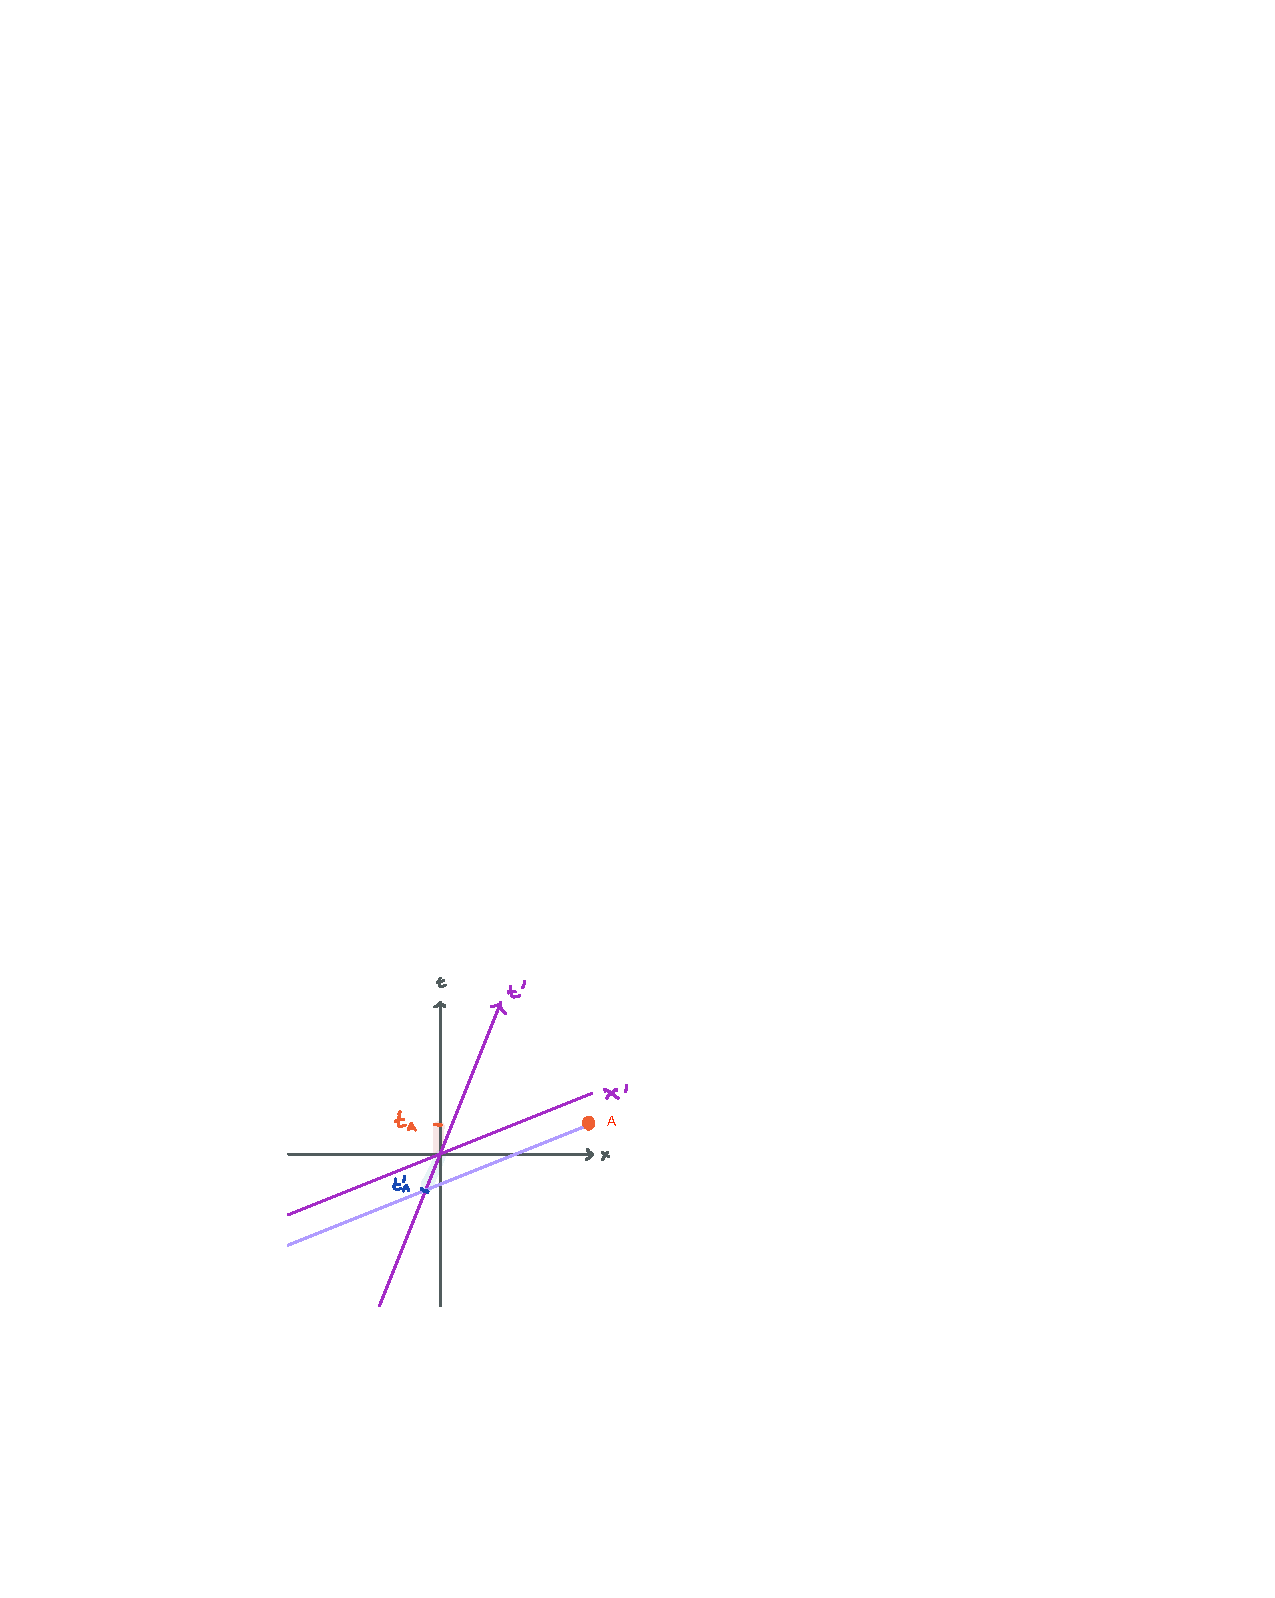
\includegraphics[width=.8\textwidth]{figures/spacetime_simultaneity.pdf}
    \captionsetup{font={scriptsize,sf}}
    \caption{Frames $(t,x)$ and $(t',x')$ are boosted relative to one another, but they agree on the origin. The unprimed observer sees event $A$ occurring \emph{after} $t=0$ while the primed observer observes $A$ occurring \emph{before} $t'=0$.}
    \label{fig:simultaneous:not}
\end{marginfigure}
What do the paradoxes of simultaneity teach us about causality? We learn that any events that occur at \emph{sufficiently} far away distances have \emph{ambiguous time ordering}. In Figure~\ref{fig:simultaneous:not} we plot the coordinates seen by two observers in relative motion, but who agree on the origin. An event, $A$, is shown as a red dot. The two observers disagree on whether the event occurs before or after the synchronization event at 0. Weird! Confirm that this is the same effect that we saw in the pole-in-barn problem.

What defines what is \emph{sufficiently} far away? This is based on an idea called the \textbf{light cone}\index{light cone}. See Figure~\ref{fig:lightcone}.
\begin{figure}[ht]
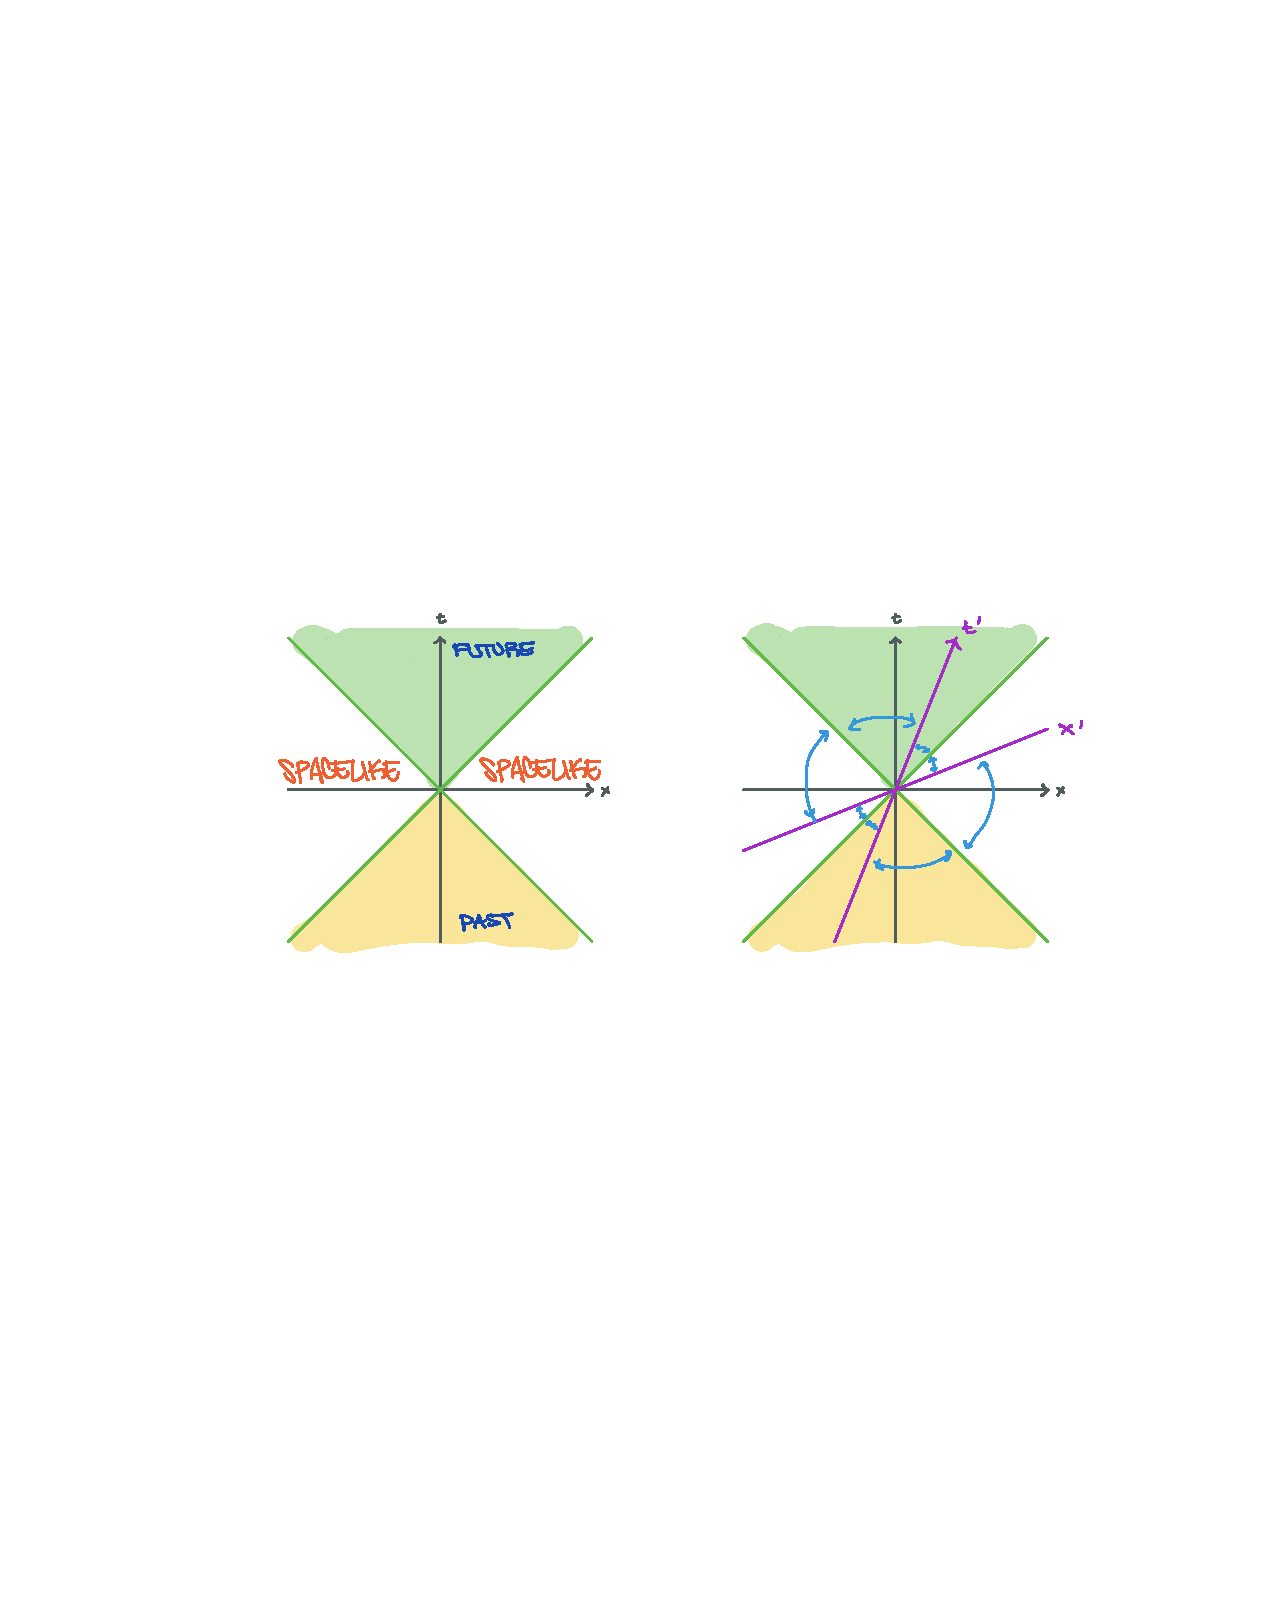
\includegraphics[width=.8\textwidth]{figures/spacetime_lightcone.pdf}
\captionsetup{font={scriptsize,sf}}
    \caption{Left: The green lines are lightcones: these are the trajectories of particles traveling at the speed of light. If you include additional spatial directions, the green lines form a conical surface of revolution. The green shaded region is the future lightcone. The yellow region is the past lightcone. The unshaded regions are spacelike separated from the origin. Right: When we show the coordinate axes observed by a boosted observer, we notice that the boosted observer agrees on the lightcones. In blue we show arrows to highlight that the lightcones are equidistant from either axis. This means that timelike and spacelike regions are maintained under Lorentz transformations.}
    \label{fig:lightcone}
\end{figure}
The lightcone is the set of possible trajectories of a particle traveling at the speed of light that passes through the origin. In more than one spatial dimension, it is a surface of revolution and hence a cone around the time axis. Any event that is closer to the time axis than the space axis---the shaded regions of Figure~\ref{fig:lightcone}---are said to be \textbf{timelike separated}\index{timelike} from the origin. This means that in \emph{any} reference frame there is a well defined ordering: if the event is in the green shaded region, every observer agrees that it occurs \emph{after} the synchronized point at the origin.\sidenote{Recall that boosts are isometries that preserve the origin---as required by linearity. Physically this means that the two reference frames have synchronized their clocks and rulers so that the zeros are synchronized at the same spacetime point.} On the other hand, events that are \textbf{spacelike separated}\index{spacelike} from the origin can either be observed as happening before, after, or synchronously with the origin \emph{depending on the observer}. Events that are on the lightcone remain on the lightcone in any frame and are called \textbf{lightlike separated}\index{lightlike separated}.

The restriction of causality then tells us that the physics of the present can only depend on events in the past lightcone and can only influence events in the future lightcone.\sidenote{In fact, causality really tells us that on a microscopic level, all interactions occur on the lightcone.} Ultimately this is a statement that the laws of physics must be \emph{local}: the microscopic laws of physics cannot depend on what is going on some finite distance away. This is why all of your favorite `laws of physics' are written as \emph{derivatives}. Derivatives are the infinitesimal separation of two points in spacetime. When the underlying laws of physics are written this way, it guarantees that you do not end up with a break in causality.

\begin{bigidea}[Causality and derivatives]\label{idea:causality:and:derivatives}
The reason why equations of motion in physics are all \emph{differential equations} is that we assume that the laws of physics must be causal, which in turn implies that the description of physics can at most depend on infinitesimal separations in space. This means that our Lagrangians are written with derivatives and hence the functional variations of these Lagrangians yield differential equations.
\end{bigidea}

\begin{exercise}[The length of a Minkowski space vector]
In Euclidean space, any vector with non-zero components has positive length-squared. In Minkowski space the length-squared can be positive, zero, or negative. This is clear from \eqref{eq:minkowski:length:2d}. In the $v^0$--$v^1$ plane, constant values of $|\vec{v}|^2$ correspond to hyperbolas. Plot the hyperbolas of points that correspond to $\vec{v}^2 = \pm 1$ and $0$. The null case, $|\vec{v}|=0$, correspond to the lightcone. In our metric sign convention, $|\vec{v}|>0$ corresponds to a timelike vector and $|\vec{v}|<0$ corresponds to a spacelike vector. Each connected component of the hyperbolae represent all of the possible components that a given vector can be observed to have by observers in different reference frames.
\end{exercise}


\section{Not all frames are inertial}

One of my favorite paradoxes in relativity is the twin paradox. Take a pair of twins. One of them becomes an astronaut and gets into a rocket ship where they travel at relativistic speeds to a nearby galaxy and then returns to Earth. The other twin remains on Earth. To the rocket-faring twin, it is the Earthbound twin who has traveled relativistically (along with the planet) before returning to meet their rocket ship. To the Earthbound twin, it is the astronaut who has been traveling relativistically. Each twin, then, would invoke the phenomenon of time dilation and would expect the other to be much younger when they reunite. Given that the two twins have equivalent reference frames, which one is older and which one is younger? 

Unlike the simultaneity puzzle, the twins are at the same spacetime point when they leave one another and they return to the same spacetime point when they compare ages.
The puzzle here is really about what breaks the asymmetry between the two frames. The resolution of the puzzle is that the space-bound twin is not in an \emph{inertial} frame: at some point their rocket has to decelerate, stop, then turn around to return to Earth. 
\begin{exercise}
Given that I have spoiled the big idea, determine which of the two twins has aged more.
\end{exercise}
\begin{exercise}
What if the universe were closed? This means that the universe is like the classic arcade game \emph{Asteroids} or \emph{Pac-Man}: if you travel too far in one direction, you end up on the other end of the screen. This is a universe that is still \emph{flat}, but has \emph{periodic boundary conditions}. In this case, the twin in the rocket ship does not need to decelerate. Then they can keep going around the universe until they meet their Earthbound twin again. This is indeed a valid inertial frame.

\textsc{Solution}: See Jeffrey Weeks' article in \emph{The American Mathematical Monthly} in 2001.\autocite{weeks:twin:doi:10.1080/00029890.2001.11919789} I am surprised that it took until 2001 for someone to have written up a solution to this problem---no doubt this was influenced by the resurrection of extra dimensions in 1998 as a potential solution to problems in particle physics. Because the resolution appeared in a professional journal analogous to our \emph{American Journal of Physics}, not many physicists seem to have known about this resolution and there were several papers after 2001 that re-discovered the same result.
\end{exercise}

It is a common refrain that acceleration cannot be accounted for in special relativity. This is formally incorrect. Like the treatment of acceleration in Newtonian mechanics, it is a bit more difficult than the simple case with no acceleration. There is, however, a reason why one may be itchy not to dwell too much on accelerated frames in special relativity. The great leap between special and general relativity comes from the realization that an accelerated observer feels forces that are identical to those of gravity. It is a much smaller leap to the identify these two ideas. We leave that for a proper exploration of general relativity.\sidenote{As a particle physicist, I would be remiss if I did not further remark that all other fundamental forces can similarly be endowed with a geometric interpretation. This geometric picture called \emph{gauge theory} is at the heart of active research in fundamental physics.}



\begin{subappendices}

\section{Relativity by Thought Experiment}\label{sec:subappendix:relativity}
You can derive special relativity from the assumption that the speed of light is constant in any reference frame and then doing so called \emph{gedankenexperiments}.\sidenote{`Thought experiments' in German.} We continue our convention of using natural units where $c=1$, though it should be obvious that using any other units just throws in factors of $c$ all over the place.
\begin{exercise}
Rewrite all the equations in this appendix with the appropriate factors of $c$. Stop when it becomes obvious how to do this. 
\end{exercise}
I first saw this done in Chapter 15 of \emph{The Feynman Lectures on Physics}\footnote{\url{https://www.feynmanlectures.caltech.edu/I_15.html}}\sidenote{\emph{The Feynman Lectures on Physics} are beloved gems of freshman-level physics insight---but the consensus is largely that they are a bit too non-sequitur in style for physics students. In fact, you come to deeply enjoy the lectures only \emph{after} you already understand most of the material---then you can appreciate the little brilliant twists that Feynman makes compared to the usual pedagogy.} I refer you to that resource for a systematic derivation from the \emph{gedanken} approach. In this appendix, follow the the general idea and focus on a few subtle points that are not often explained carefully in the standard literature.\sidenote{I thank Matthew Lugatiman and Adam Green for talking through some of these subtleties with me.}

Just as the word \emph{gedankenexperiment} tells you where special relativity was developed, so too does the standard setting of the \emph{gedankenexperiment}: start by imagining a train moving with some velocity $v=\beta$ in the $x$ direction relative to our coordinate system. We are \emph{outside} the train. We are observers, $\mathcal O$ and our coordinate system is $(t,x)$. You can also imagine another observer, Oppie,\sidenote{This is \emph{not} a reference to Oppenheimer's nickname or a misspelling of Opie, Ron Howard's most famous character. Instead, it's a name that is reasonably close to $\mathcal O'$, ``oh-prime.''} who is \emph{in} the train and whose coordinate system carries primes: $(t',x')$. We say that Oppie is a \emph{comoving} observer with the train. We align our coordinate systems so that the origins coincide: 
\begin{align}
    (t=0,x=0) = (t'=0,x'=0) \ .
\end{align}
The above equation should be treated to mean \emph{the point that we call $(0,0)$ coincides with the point that Oppie calls $(0,0)$.} In this way, a generic point $(t,x)$ is really a \emph{separation} between that point and the origin.\sidenote{Recall our caveat in Section~\ref{sec:no:position:vectors}: positions are not vectors, but differences in positions are vectors.}


\subsection{Time dilation}

First imagine that Oppie has a little gizmo that first emits a photon towards a mirror, then detects the reflected photon. See Fig.~\ref{fig:Feynman:photo:thing}
\begin{marginfigure}%[th]
    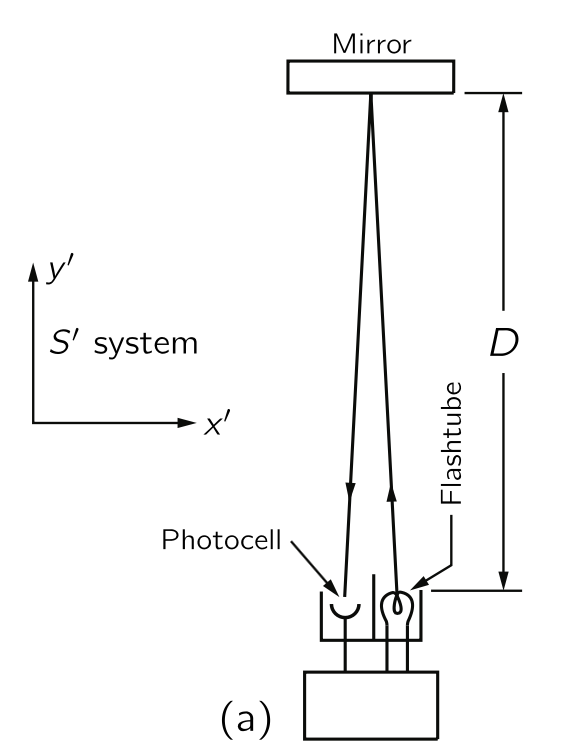
\includegraphics[width=.8\textwidth]{figures/FeynmanLec15_photodet.png}
    \captionsetup{font={scriptsize,sf}}
    \caption{From \emph{The Feynman Lectures on Physics}, Chapter 15.}
    \label{fig:Feynman:photo:thing}
\end{marginfigure}
The height of the gizmo is $D = \ell$, the height of the train. It is critical that the gizmo is aligned so that the photon moves \emph{perpendicular} to the direction of motion. We write $\ell$ for \emph{length} and to avoid ambiguities with [covariant] derivatives, $D$ mesons, and so forth. 

Like us, Oppie understands that the speed of light is $c=1$ and that this is true in any reference frame. At the origin ($t'=0$), Oppie turns ont he gizmo and measures the time $t'$ that it takes for the photon to traverse the distance $\ell$ and come back. 
\begin{align}
     t' = 2\ell/c = 2\ell \ .
     \label{eq:Feynman:train:updown}
\end{align}

What do we see? Like Oppie, we see the device turn on at the origin ($t=0$) and we see that the photon hits the roof of the train car and bounces back down. However, unlike Oppie, we also see the entire system move in direction of the train's motion. The trajectory is shown in Fig.~\ref{fig:Feynman:photo:thing:unprimed}.
\begin{figure}[ht]
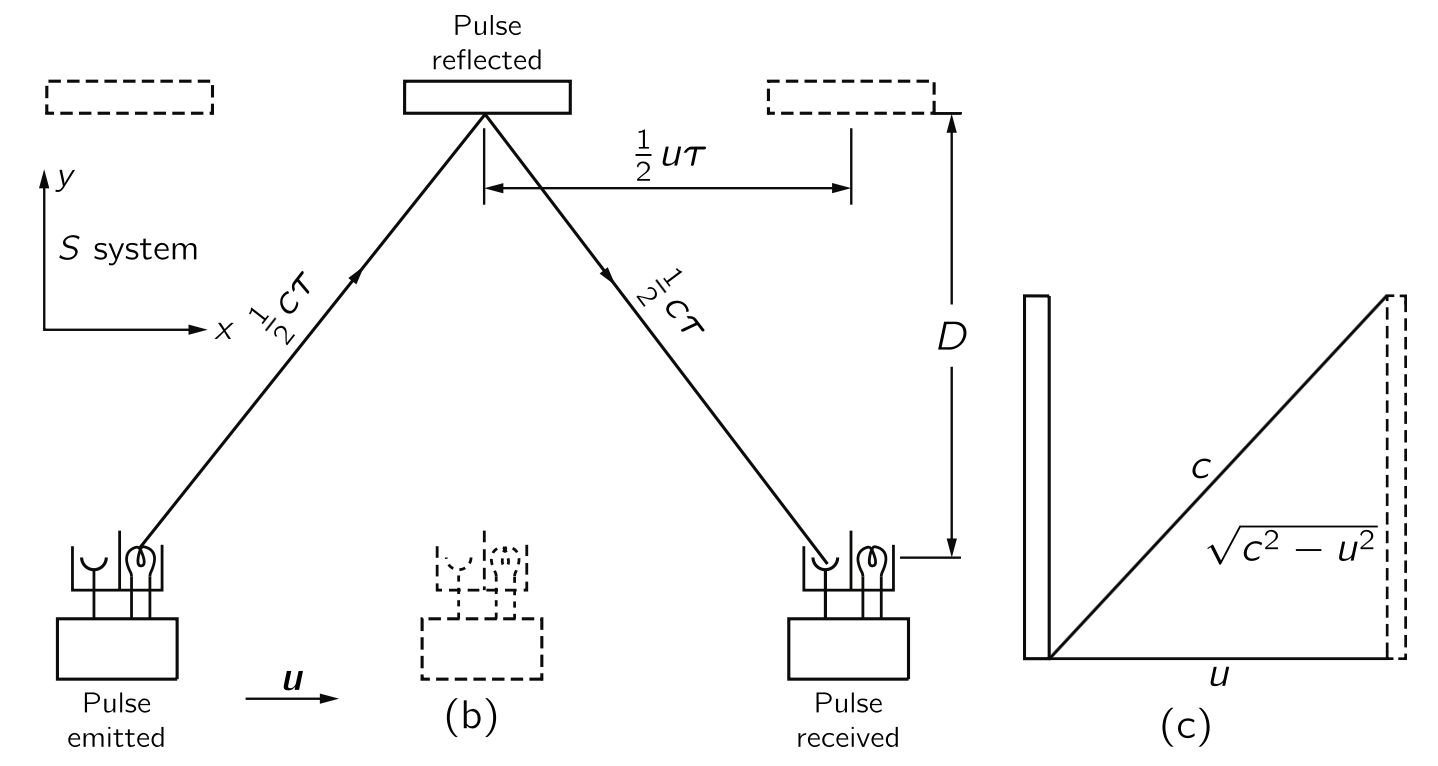
\includegraphics[width=\textwidth]{FeynmanLec15_photodetside.png}
    \captionsetup{font={scriptsize,sf}}
    % \caption
    \sidecaption[][-7em]{Same as Fig.~\ref{fig:Feynman:photo:thing}, but as seen from observers who are not on the train. From \emph{The Feynman Lectures on Physics}, Chapter 15.
    \label{fig:Feynman:photo:thing:unprimed}
    }
\end{figure}
Because the motion of the train is perpendicular to the up-and-down direction, we assume that the height of the train is unchanged by relativistic effects: we measure this height to be $\ell$ just as Oppie does. We then measure that the photon takes times $t$ to hit the top of the train and return. This time is evenly split\sidenote{By symmetry.} between the upward-going time and downward-going time. During this time, the train has moved along the $x$ direction by an amount $\beta t$. From trigonometry, we thus have:
\begin{align}
    \left(\frac{t}{2}\right)^2
    &= 
    \left(\frac{\beta t}{2}\right)^2 + \ell^2
\end{align}
Plugging in Oppie's observation that that relates the height of the train to the time Oppie measures, \eqref{eq:Feynman:train:updown}, we have
\begin{align}
    (t')^2 = (1-\beta^2) t^2 =  \frac{t}{\gamma} \ .
\end{align}
That is to say, the time that we measure is related to the time that Oppie measures by
\begin{align}
    t = \gamma t' \ .
    \label{eq:time:dilation:derived}
\end{align}
Because $\gamma > 1$, we the time that we see is \emph{dilated} relative to what Oppie experiences. Because the gizmo is essentially an idealized clock, we say that observers see the events on the moving train moving  slower than they would expect by a factor $\gamma$. 




\subsection{Length contraction}

Having learned something about the passage of time, we can now figure out what motion does to the relative perception of space. To do this, let us do a second experiment where we turn the gizmo in Fig.~\ref{fig:Feynman:photo:thing} onto its side. Place the gizmo at the back of a train car and arrange it so that the photon first moves \emph{along the direction of the train's motion}, then reflects off of the mirror to go \emph{against the direction of the train for its return motion}. Let us now set the length of the gizmo to be the length of the train car: Ollie observes\sidenote{We write $\ell_0$ rather than $\ell'$ because Ollie is in the rest frame of the train. $\ell_0$ is called a \emph{proper length}, it is the length of an object to an observer for whom the object is not moving.} this to be $\ell_0$ while we observe it to be $\ell$. 

In pre-special relativity Galilean physics we would expect $\ell_0 = \ell$. However, the fact that $c=1$ is constant means that we cannot make this assumption. 
\begin{marginfigure}%[th]
    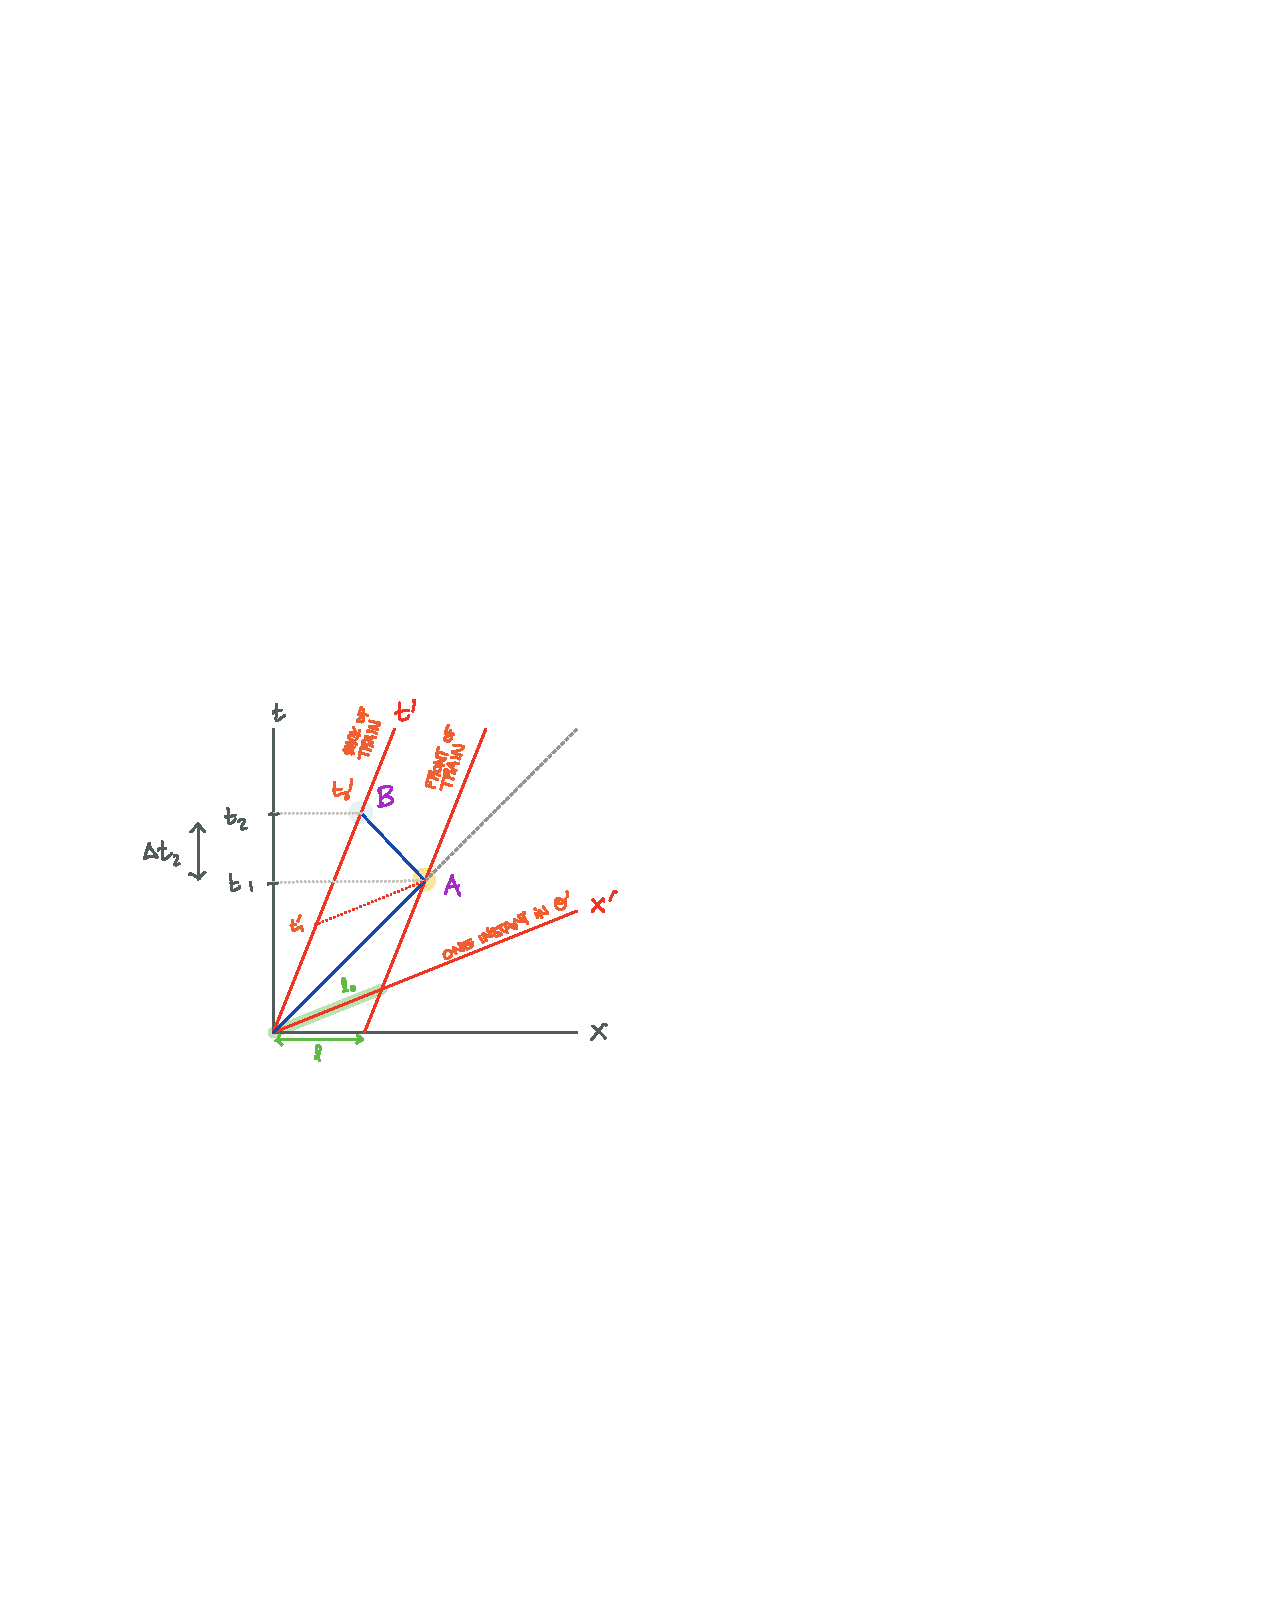
\includegraphics[width=\textwidth]{figures/spacetime_lengthcontraction.pdf}
    \captionsetup{font={scriptsize,sf}}
    \caption{The trajectory of the photon (dark blue) from the back of the train at $t=t'=0$ to the event $A$ then the event $B$ where it returns to the back of the train. Oppie's coordinate system is in red. \label{fig:spacetime:length:diagram}}
\end{marginfigure}
Points on a spacetime diagram are called \emph{events} because they are a place and a time. Figure~\ref{fig:spacetime:length:diagram} shows the experiment. Let the origin be the back of the train at time zero---where both we and Oppie synchronize our clocks. A photon is shot towards the end of the train. The two edge of the train correspond to the $t'$ axis and its parallel translation---this is because in Oppie's frame the train is not moving and so it stays at $x'=0$; similarly, the front of the strain stays at $x'=\ell_0$. 

The photon travels at the speed of light $c=1$, which is a 45$^\circ$ diagonal line on the way out, then a 135$^\circ$ line on the way back. The thought experiment is again simpler in Oppie's frame. Oppie measures that the total time for the back-and-forth journey is $t_2' = 2\ell'$. It is clear both from the thought experiment and the diagram that each leg of the journey takes the same amount of time $t_2' = 2t_1'$.

We see something a bit different. On the outbound journey the photon has to \emph{catch up} to the front train. If we could observe it, we would measure that it takes time $t_1$ for the photon to reach the mirror. After it reflects off the mirror at the front of the train, the photon and the back of the train are moving \emph{toward each other}. We observe that this total journey takes a time $t_2$. We also define $\Delta t_2 = t_2 - t_1$ to be just the time of the journey from the front of the train to the back again. Observe that $\Delta t_2 \neq t_1$; both logically and from Figure~\ref{fig:spacetime:length:diagram}. This means we have the relations:
\begin{align}
t_1 &= \ell + \beta t_1
&
\Delta t_2 &= \ell - \beta \Delta t_2 \ .
\end{align}
Here we recall that $\beta$ is the speed of the train and the different signs correspond to whether the train is moving with or against the photon. Since $t_1$ is already measured against the origin, there is no need to write $\Delta t_1 \equiv t_1 - 0 = t_1$. These give us the relations:
\begin{align}
    (1-\beta)t_1 &= \ell & (1+\beta)\Delta t_2 &= \ell
    \ .
\end{align}
The total time is then
\begin{align}
    t_2 = t_1 + \Delta t_2 = \frac{\left[(1 + \beta) + (1-\beta)\right]\ell}{1-\beta^2}
    = 2\gamma^2 \ell \ .
    \label{eq:gedanken:length:intermediate1}
\end{align}
\begin{exercise}
Prove \eqref{eq:gedanken:length:intermediate1}. It is worth doing.
\end{exercise}
Now we have to invoke time dilation in \eqref{eq:time:dilation:derived}. The total time for the round trip journey that we measure $t_2$ is related to the total time that Oppie measures $t_2'$ by
\begin{align}
    t_2 &= \gamma t_2'
    \\
    2\gamma^2 \ell &= 2\ell' 
    \\
    \ell = \frac{\ell'}{\gamma}
    \label{eq:length:contraction:derived}
    \ .
\end{align}
Because $\gamma > 1$, we find that what \emph{we} measure to be the length of the train is \emph{contracted} (smaller) relative to what Oppie measures in the comoving frame of the train.


\subsection{Confusion}

The lessons of this \emph{gedanken} appendix are simple. If the frame $\mathcal O'$ is moving relative to our frame, $\mathcal O$, then
\begin{itemize}
    \item From \eqref{eq:time:dilation:derived}: The time that we measure is \emph{dilated} (slower) compared to the time that is measured in $\mathcal O'$. 
    \item From \eqref{eq:length:contraction:derived}: Length along the direction of motion are \emph{contracted} (smaller) compared to the length along the direction of motion measured in $\mathcal O'$. 
\end{itemize}
Having established these, I leave it to you to explore some of the apparent paradoxes in special relativity such as the pole-in-barn paradox and the twin paradox. The spacetime diagrams that we draw are useful guides. As a hint, often the resolution to paradoxes is the observation that simultaneity is a frame-dependent notion.\sidenote{This has a manifestation for us: the locality of the fundamental interactions is a logical consequence of requiring causality in our theory. Interactions must happen at a single \emph{event} rather than over a finite separation in order for there to be a clear \emph{cause} that precedes an \emph{effect} in any valid reference frame.}

Thus far, everything we have discussed in this appendix is standard fare in a decent treatment of first-year modern physics. Let us focus on some of the conceptual hiccups that are not always explained carefully.

\paragraph{Could we derive length contraction without using time dilation?} You should feel unsatisfied. In relativity, space and time have equal footing. However, \emph{every} thought-experiment based derivation of special relativity starts by deriving time dilation and \emph{then} uses that result to derive length contraction. The reason for this asymmetry is that the time dilation thought experiment did not depend on the directions perpendicular to the train's motion: both the $\mathcal O$ and $\mathcal O'$ frame measured the height of the train to be $\ell$. On the other hand, the length contraction thought experiment had both spatial displacement $\ell$ \emph{and} a time displacement $t_2$ that needed to be measured in each reference frame. To say it differently: the time dilation experiment allowed us to ignore part of the spatial configuration. However, in the length contraction experiment you \emph{cannot} ignore the time separation because all experiments evolve in time.\sidenote{Philosophically: we perceive the universe as a sequence in time. We can imagine experiences where we are stationary in space, but we have no experiment---\emph{gedanken} or otherwise---where we are stationary in time.} Rest assured, the geometry \emph{does} respect the symmetry between space and time.

\paragraph{If they are so useful, why did we not draw a spacetime diagram for the time dilation experiment?} The time dilation experiment made use of a third dimension of spacetime, the height of the train. It is a bit of a pain to draw, and you still end up drawing the same right triangles in Fig.~\ref{fig:Feynman:photo:thing:unprimed}


\paragraph{Was it necessary for the photon to complete a full loop?} In these thought experiments, the the photon is emitted and detected by the same device: the trajectory is an `out and back' in runners parlance. For the time dilation experiment, it is obviously sufficient to consider only the trajectory from the origin to the ceiling. What about for the length contraction experiment? This is also possible. 
\begin{exercise}
Derive time dilation using the same thought experiment, but without the `return journey' to the back of the train. 
\end{exercise}
That this is possible is obvious for those with experience with relativity. However, it is useful pedagogically to have the photon perform a round trip journey because this way all observations are performed by the same observer. I can say that \emph{Oppie} emits a photon and \emph{Oppie} observes its return. Then we can identify the event where we observe Oppie emitting a photon and the event where we observe Oppie observing the photon.\sidenote{Given the subtleties of spacetime separated events with regard to simultaneity, I can appreciate this pedagogical choice.}

\paragraph{I tried calculating this using Lorentz transformations and I got stuck.} Here is a common error. Suppose we know that Oppie measures the train car to have length $\ell_0$ and that Oppie measures this at some time slice $t'=0$. Then we can perform a Lorentz transformation:
\begin{align}
    \begin{pmatrix}
        t\\
        \ell
    \end{pmatrix}
    =
    \begin{pmatrix}
        \gamma &\gamma\beta\\
        \gamma \beta & \gamma
    \end{pmatrix}
    \begin{pmatrix}
        0\\
        \ell_0
    \end{pmatrix}
    = 
    \begin{pmatrix}
        \gamma\beta\ell_0
        \gamma \ell_0
    \end{pmatrix} \ .
\end{align}
From this we believe that $\ell = \gamma \ell_0$, i.e.\ length is \emph{also} dilated---which is \emph{incorrect}! What went wrong here? Recall that the \emph{event} that we are using to measure the length of the train is a photon hitting the back of the train. That is labeled event $A$ in Fig.~\ref{fig:spacetime:length:diagram}. This occurs on the light cone where $t=x$ (and also $t'=x'$). That means that we need to Lorentz transform the separation between the \emph{event} $(t_1'=\ell_0, x'=\ell_0)$. This gives
\begin{align}
    \begin{pmatrix}
        t_1\\
        \ell
    \end{pmatrix}
    =
    \begin{pmatrix}
        \gamma &\gamma\beta\\
        \gamma \beta & \gamma
    \end{pmatrix}
    \begin{pmatrix}
        \ell_0\\
        \ell_0
    \end{pmatrix}
    = 
    \begin{pmatrix}
        \gamma(1+\beta)\ell_0\\
        \gamma(1+\beta)\ell_0
    \end{pmatrix} 
    \ .
\end{align}
We can use the first component and our time dilation result to find:
\begin{align}
    t_1 \equiv \ell &= \gamma (1+\beta)(1-\beta) \ell' 
    \\ &= \frac{\ell'}{\gamma}
    \ .
\end{align}
We have used the definition that $\gamma = (1-\beta^2)^{-1}$. 
From this we indeed confirm $\ell = \ell'/\gamma$ and that length is \emph{contracted}. 




\section{More examples in relativity}

\subsection{%Example: 
The electromagnetic field strength}
% motivate this from the unification of magnetism and electricity
% transformation laws

\begin{figure}[tb]
    \centering
    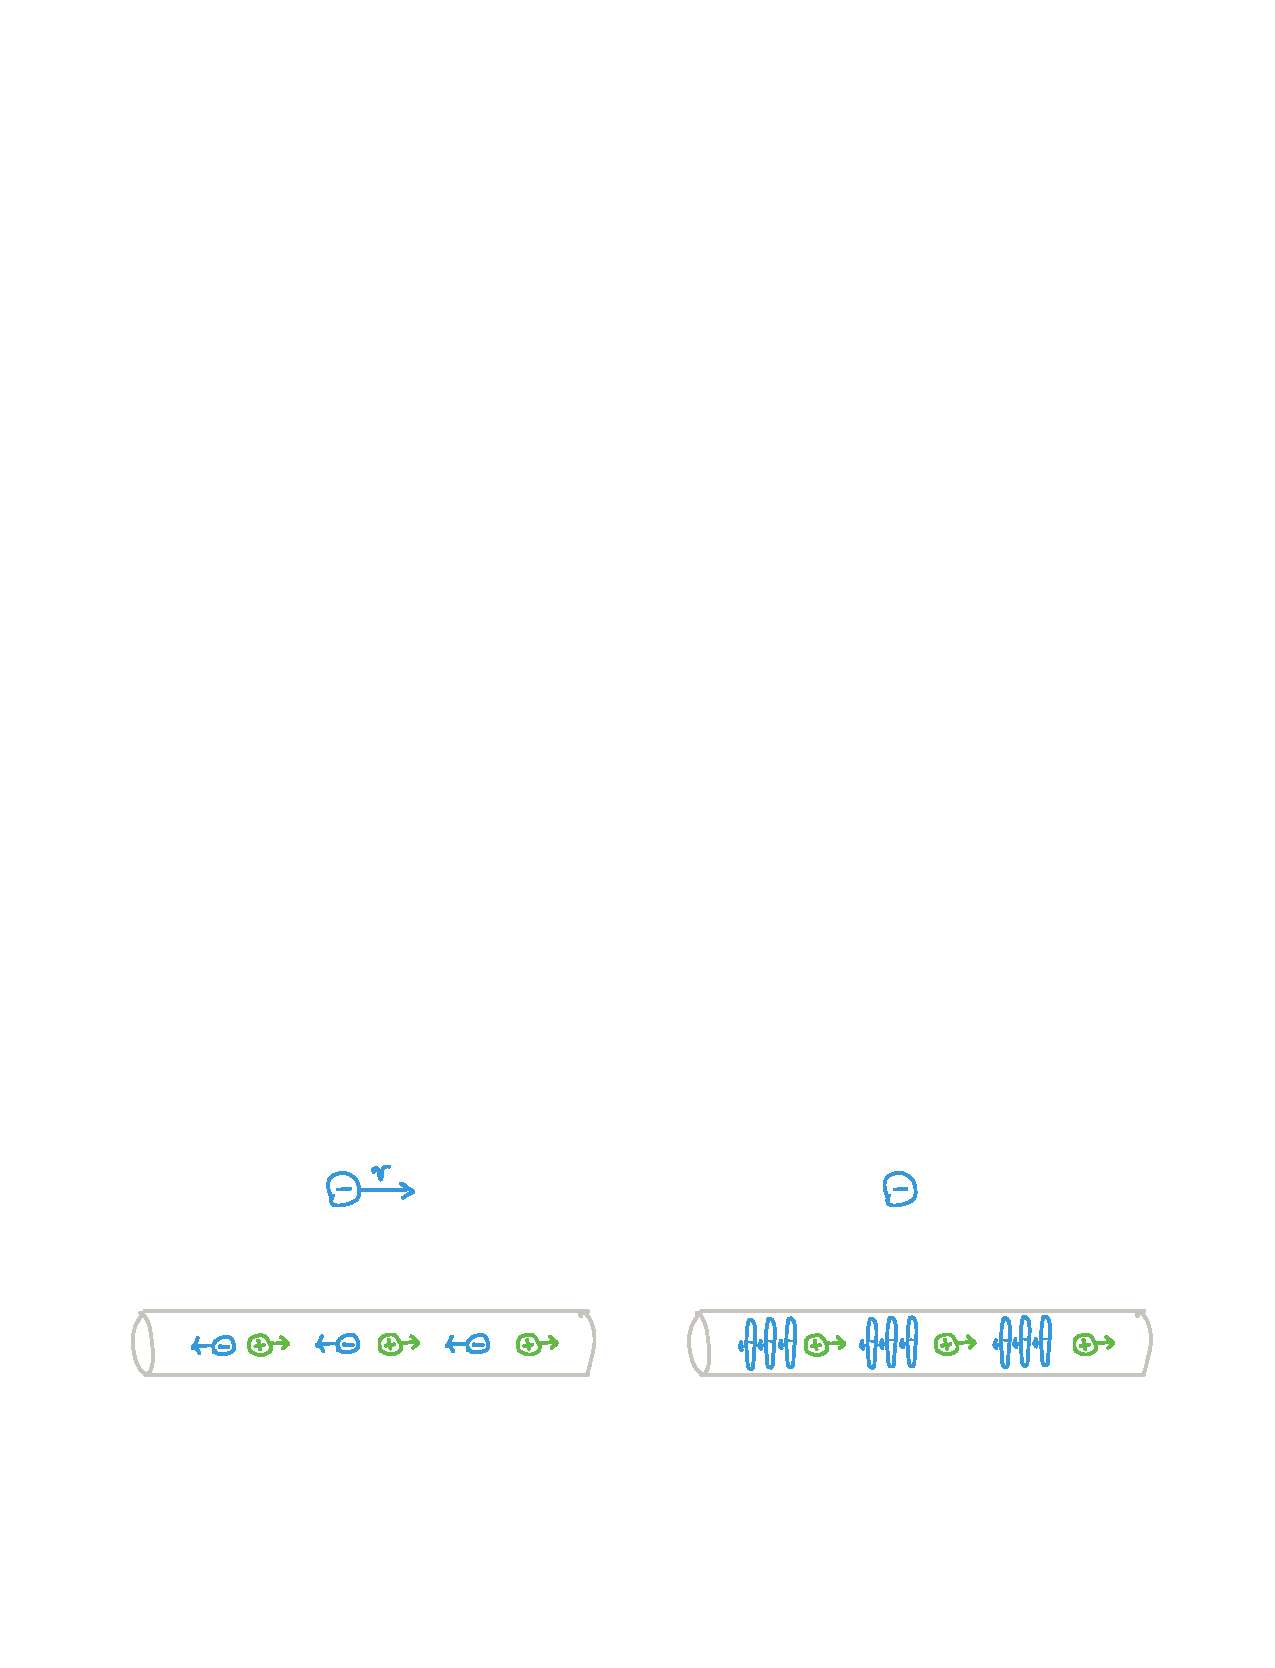
\includegraphics[width=\textwidth]{figures/EMcurrent.pdf}
    \caption{\textsc{Left}: an electron moves near a current. The current has no net electric charge. In the absence of magnetism, we expect the electron to move in a straight line. \textsc{Right}: if we boost into the electron frame, the particles in the current moving in the opposite direction are length-contracted. This means that the charge density increases. The stationary electron now feels a net electric force. This implies that something is missing in the picture on the left.}
    \label{fig:current}
\end{figure}

Another place where special relativity rears its head is in electrodynamics. Electricity and magnetism are two manifestations of the same electromagnetic phenomenon.\sidenote{Unification of apparently unrelated forces is a big theme of this course. Electromagnetism is the example that you already know.} This is illustrated in Fig.~\ref{fig:current}. If you did not know about magnetism, you would find a paradox when you consider a charged particle moving along a current. In one frame, the current is an equal number of positive and negative charges moving in opposite directions.\sidenote{I suppose more realistically the negative charges move while the positive charges stay put---that does not change the conclusion.} If you boost to the external charged particle's rest frame, length contraction forces one species of the current particles to increase their charge density relative to the other species. This creates a net electric field that acts on the stationary external particle. Without magnetism, the first frame is missing this additional force. 

The electric and magnetic fields are unified in the \emph{electromagnetic field strength}, which is a two-index tensor:
\begin{align}
    F^{\mu\nu}
    &=
    \begin{pmatrix}
        0&-E^x&-E^y&-E^z\\
        E^x&0&-B^z&B^y\\
        E^y&B^z&0&-B_x\\
        E^z&-B^y&B^x&0
    \end{pmatrix} %\ .
    \\
    F_{\mu\nu}
    &=
    \begin{pmatrix}
        0&E^x&E^y&E^z\\
        -E^x&0&-B^z&B^y\\
        -E^y&B^z&0&-B_x\\
        -E^z&-B^y&B^x&0
    \end{pmatrix} \ .
    \label{eq:fmunu:lower}
\end{align}
We see that electricity and magnetism are unified in that their components mix into one another under a Lorentz transformation. 
\begin{exercise}
Confirm that $F_{\mu\nu} =g_{\mu \alpha}g_{\nu\beta} F^{\alpha\beta}$ with the (3+1)-dimensional Minkowski metric $g_{\mu\nu}$. 
\end{exercise}
\begin{exercise}
Find the components of $F'^{\mu\nu}$ under a boost along the $z$-direction. 
\end{exercise}


\subsection{%Example: 
Simultaneity}
\label{eq:simultaneity}

One of the key ideas in special relativity is that we sacrifice our notion of simultaneity for objects that are not observed at the same spacetime point. We may reuse our diagram in Fig.~\ref{fig:re:dilation}. Consider two different points on the $x'$ axis. These are simultaneous with respect to the primed observer: they both occur at $t'=9$. However, these two points  obviously do \emph{not} have the same $t$ coordinate to the unprimed observer. This observation helps clear up several apparent paradoxes that may show up in relativity. More importantly, it completely upends our notion of causality.

One of the unwritten-but-understood laws of physics is that the cause precedes the effect. I have to drop my mug before I hear the sound of the ceramic shattering. This notion is imperiled if in some other reference frame someone else would have heard the shattering before they observe the mug being dropped. One deduction of this is that the laws of physics should be \emph{local} in spacetime. A consequence of this observation is that the laws of physics should be written with derivatives.


\subsection{%Example: 
Discrete isometries}

Isometries are symmetries of the metric.
% 
The Minkowski metric has a parity isometry that acts as a discrete symmetry. In matrix form the action of parity is a Lorentz transformation
\begin{align}
    P = \begin{pmatrix}
        1 & & &\\
         & -1& &\\
         & & -1 &\\
         & & & -1
    \end{pmatrix}\ .
\end{align}
This symmetry is \emph{discrete} in contrast to continuous symmetries. Rotations are a continuous symmetry because you can rotate by any real number amount, $\theta$. They parameterize an infinite number of Lorentz transformations. Discrete symmetries, on the other hand, represent a countable number of Lorentz transformation. In fact, because $P^2 = \mathbbm{1}$, there is only one such Lorentz transformation. 

There is a second discrete transformation called \textbf{time reversal}:
\begin{align}
    T = 
    \begin{pmatrix}
        -1 & & &\\
        & 1 & &\\
        &  & 1 &\\
        &  & & 1
    \end{pmatrix} \ .
\end{align}
This one sounds rather dramatic, doesn't it?\sidenote{One of my mentors in graduate school once told the story that he was preparing a lecture on particle physics at the pub. When his friends asked him what the topic of the lecture would be, he said ``time reversal.'' The bar crowd suddenly grew silent until the bartender quietly asked: ``... we can do that?''} It should be clear that $T$ indeed reverses the direction of time. This, however, does not mean that time reversal is something we can do.\sidenote{Time reversal is a major part of \emph{The Legend of Zelda: Tears of the Kingdom}. Before this, there was the ground-breaking independent computer game \emph{Braid} that pioneered this mechanic. The latter has an additional connection to physics in that the story is largely understood to be a parable about the development of atomic weapons.} Our understanding of causality breaks if we allow time reversal. However, mathematically time reversal is a clear isometry of the Minkowski metric. 

In fact, there is something `deep' to say that the classical laws of physics are time reversal invariant. If you run a video backwards, everything that happens obeys the laws of physics. The sign of the gravitational force may swap, but the dynamics of such an ``anti-gravity'' force law follows Newtonian mechanics. Entropy may decrease rather than increase, but there is no sense in which the microscopic transition from one configuration to the next would violate any laws of microphysics.\sidenote{This is to say that the ``arrow of time'' from statistical mechanics is not a statement about microscopic interactions nor is it a statement about what is not \emph{possible}, only about what is increasingly \emph{improbable}.} Though, to be fair, we also do not know how to take a right-handed person and do a parity transformation on them to turn them left-handed. 


In order to restrict to sensible isometries, we say that valid observers in special relativity are those that are related by isometries that are \emph{connected to the identity}. This means that one may write the isometry with respect to a continuous parameter and that for some value of that parameter, the isometry is simply the identity matrix. In this way, we restrict our physical isometries to those that maintain the direction of time. 

There is one more discrete symmetry that is often mentioned along with parity and time reversal: charge inversion. Unlike the other two, charge inversion is \emph{not} a spacetime symmetry since it acts only on particles (fields). Charge inversion takes every particle and flips their charges. For now you may think about flipping the \emph{electric} charge of the particle---but this actually holds for all of the types of charges that we examine in this course.\sidenote{Charges are conserved quantities. Remember that conserved quantities come from symmetries of the action. Unlike the spacetime symmetries of this chapter, those charges are related to \emph{internal} symmetries.} There are two combinations of these discrete symmetries that are notable:
\begin{itemize}
    \item The combination $CP$ (charge--parity) is the transformation that takes a particle to its anti-particle.
    \item The combination $CPT \equiv \mathbbm{1}$. That is: if we perform all three discrete symmetries, we return to the same state.%\sidenote{I leave this here with no proof. I know such proofs exist, but they are largely in the domain of a construction called axiomatic quantum field theory, which I know nothing about. You can learn more about this in\footnotemark}\footnotetext{\cite{Blum:2022eol}}
\end{itemize}
Because these are all parities---in the sense that $C^2 = P^2 = T^2 = \mathbbm{1}$---we see an relation between the antimatter transformation $CP$ and the idea of moving backward in time. You may want to remember then when our Feynman diagram notation makes it \emph{look like} antiparticles are particles moving backward in time.\sidenote{To be clear, this is \emph{not} what is happening.}

\end{subappendices}
